\documentclass[format=acmsmall, review=false, screen=true]{acmart}

\usepackage{booktabs} % For formal tables

\usepackage[ruled]{algorithm2e} % For algorithms
\renewcommand{\algorithmcfname}{ALGORITHM}
\SetAlFnt{\small}
\SetAlCapFnt{\small}
\SetAlCapNameFnt{\small}
\SetAlCapHSkip{0pt}
\IncMargin{-\parindent}


% Metadata Information
\acmJournal{TOMM}
%\acmVolume{1}
%\acmNumber{1}
%\acmArticle{1}
%\acmYear{2018}
%\acmMonth{11}
\copyrightyear{2019}
%\acmArticleSeq{9}

% Copyright
%\setcopyright{acmcopyright}
\setcopyright{acmlicensed}
%\setcopyright{rightsretained}
%\setcopyright{usgov}
%\setcopyright{usgovmixed}
%\setcopyright{cagov}
%\setcopyright{cagovmixed}

% DOI
\acmDOI{0000001.0000001}

% Paper history
\received{November 2018}
\received[revised]{2019}
\received[accepted]{2019}


% Document starts
\begin{document}
% Title portion. Note the short title for running heads
\title[RenderGAN]{RenderGAN: Application of encoder-decoder architecture in combination with GAN framework for Rendering generatio}

\author{Marco Mameli}
\orcid{0000-0002-5269-9939}
\affiliation{%
  \institution{Universit\`a Politecnica delle Marche, Dipartimento di Ingegneria dell'Informazione (DII)}
  \streetaddress{Via Brecce Bianche, 12}
  \city{Ancona}
  \state{}
  \postcode{60131}
  \country{Italy}}
\email{m.mameli@pm.univpm.it}

\author{Marina Paolanti}
\affiliation{%
  \institution{University of Macerata, Department of Political Sciences, Communication and International Relations}
  \streetaddress{Via Don Minzoni, 22A}
  \city{Macerata}
  \state{}
  \postcode{62100}
  \country{Italy}
}
\email{marina.paolanti@unimc.it}

\author{Adriano Mancini}
\orcid{0000-0001-5281-9200}
\affiliation{%
  \institution{Universit\`a Politecnica delle Marche, Dipartimento di Ingegneria dell'Informazione (DII)}
  \streetaddress{Via Brecce Bianche, 12}
  \city{Ancona}
  \state{}
  \postcode{60131}
  \country{Italy}
}
\email{a.mancini@univpm.it}

\author{Rocco Pietrini}
\orcid{0000-0003-4343-7555}
\affiliation{%
  \institution{Universit\`a Politecnica delle Marche, Dipartimento di Ingegneria dell'Informazione (DII)}
  \streetaddress{Via Brecce Bianche, 12}
  \city{Ancona}
  \state{}
  \postcode{60131}
  \country{Italy}
}
\email{r.pietrini@staff.univpm.it}

\author{Primo Zingaretti}
\affiliation{%
  \institution{Universit\`a Politecnica delle Marche, VRAI - Vision Robotics and Artificial Intelligence Lab, Dipartimento di Ingegneria dell'Informazione (DII)}
  \streetaddress{Via Brecce Bianche, 12}
  \city{Ancona}
  \state{}
  \postcode{60131}
  \country{Italy}
}
\email{p.zingaretti@staff.univpm.it}


\begin{abstract}
In the domain of computer graphics, achieving high visual quality in real-time rendering remains a formidable challenge due to the inherent time-quality trade-off. Conventional real-time rendering engines sacrifice visual fidelity for interactive performance, while image generation using path-tracing techniques can be exceedingly time-consuming. In this paper, we introduce RenderGAN, a cutting-edge deep learning-based solution designed to address this critical challenge in real-time rendering. RenderGAN utilizes G-Buffers and information from a real-time rendering engine as inputs to produce output images with exceptional visual fidelity. Its encoder-decoder architecture, trained using the Generative Adversarial Network (GAN) framework with perceptual loss, enhances image realism. To evaluate RenderGAN's effectiveness, we quantitatively compare the generated images with those of a path-tracing engine, obtaining a remarkable Universal Image Quality Index (UIQI) value of 0.898. RenderGAN's open-source nature fosters collaboration, driving advancements in real-time computer graphics and rendering techniques. By bridging the gap between real-time and path-tracing rendering, RenderGAN opens new horizons for accelerated image generation, inspiring innovation and unlocking the full potential of real-time visual experiences.
\end{abstract}


%
% The code below should be generated by the tool at
% http://dl.acm.org/ccs.cfm
% Please copy and paste the code instead of the example below.
%
\begin{CCSXML}
<ccs2012>
   <concept>
       <concept_id>10003033.10003034.10003035.10003036</concept_id>
       <concept_desc>Networks~Layering</concept_desc>
       <concept_significance>300</concept_significance>
       </concept>
 </ccs2012>
\end{CCSXML}

\ccsdesc[300]{Networks~Layering}

%
% End generated code
%
\keywords{}




\maketitle

% The default list of authors is too long for headers.
\renewcommand{\shortauthors}{M. Mameli et al.}

\section{Introduction}
\label{sec:introduction}
Computer graphics (CG) has revolutionized numerous fields, enabling the creation of visually stunning digital content~\cite{mamurova2023role}.
In this dynamic and constantly evolving field, achieving real_time rendering with uncompromising visual quality remains an elusive challenge. The demand for high_fidelity images in real_time applications, such as video games, simulations, and virtual reality experiences, has led to a pressing need for innovative solutions that address the time_quality trade_off. Achieving high visual quality in CG remains a complex task, particularly when time is of the essence~\cite{agoston2005computer}. One critical aspect of CG lies in rendering a 3D scene into an image, a process that demands substantial computing resources and time~\cite{peresunko2021models}. The rendering operation plays a pivotal role within the simulation context, and it encompasses two main techniques: real_time rendering and path_tracing rendering. Real_time rendering offers rapid image generation but compromises on the intricate details that contribute to visual realism. In contrast, path_tracing rendering produces images of exceptional quality, considering shadows, lighting, and material intricacies, but at the cost of substantial time investment. Bridging the gap between real_time and path_tracing rendering is a longstanding challenge that has profound implications across various domains~\cite{wu2020analytic}.

In response to these challenges, Deep learning has emerged as a transformative force in the realm of real_time rendering, revolutionizing the way we approach the age_old challenge of achieving high visual quality with limited computational resources~\cite{xiao2020neural}. Traditionally, real_time rendering has grappled with the trade_off between speed and visual fidelity, often sacrificing the latter for interactive performance. However, the advent of deep learning techniques, such as Generative Adversarial Networks (GANs)~\cite{goodfellow2020generative} and convolutional neural networks (CNNs), has opened up new possibilities for accelerating image generation without compromising on realism. By training encoder_decoder architectures on huge datasets of rendered images, deep learning models can now approximate the intricate details of scenes and produce visually compelling result in real_time~\cite{shi2021towards}. From video games to virtual reality experiences, the integration of deep learning in real_time rendering has not only elevated visual quality but also unlocked innovative approaches to bridging the gap between real_time and offline rendering techniques. By harnessing the power of convolutional networks and leveraging images generated by real_time engines, it becomes possible to generate output images that closely resemble those produced by path_tracing engines. This convergence of deep learning and real_time rendering has the potential to revolutionize the field, opening up new possibilities for accelerated image generation in CG~\cite{shi2021towards}.

Considering this context, in this paper it is introduced RenderGAN, a groundbreaking deep learning_based solution tailored to tackle the time_quality trade_off in real_time computer graphics. By leveraging G_Buffers and information from a real_time rendering engine, RenderGAN generates output images with extraordinary visual fidelity. Its encoder_decoder architecture, trained using the GAN framework with perceptual loss, enhances the realism of the generated images. Through rigorous quantitative comparisons with path_tracing engine result, RenderGAN achieves an impressive Universal Image Quality Index (UIQI) value of 0.898. Additionally, visualizations demonstrate the striking resemblance between RenderGAN's rendered images and those produced by path_tracing engines. What sets RenderGAN apart is its commitment to openness, encouraging collaboration, innovation, and accessibility within the computer graphics community. Unlike proprietary alternatives, RenderGAN fosters collective efforts to advance real_time computer graphics and rendering techniques, benefiting diverse applications and industries. By seamlessly merging deep learning and real_time rendering, RenderGAN opens up new avenues for accelerated image generation, bridging the gap between real_time and path_tracing rendering. The remarkable reduction in rendering time, without compromising visual quality, promises to revolutionize real_time computer graphics, propelling innovation in this dynamic and ever_evolving field. RenderGAN's open_source nature empowers researchers and practitioners to explore the forefront of accelerated image generation, driving the future of real_time rendering and fostering a collaborative, forward_thinking community.

The main contributions of this paper are as follows: i) the design of RenderGAN, a novel deep learning_based solution that addresses the time_quality trade_off in real_time computer graphics. RenderGAN uses G_Buffers and information from a real_time rendering engine as inputs to generate output images with remarkable visual fidelity; ii) presenting an innovative encoder_decoder architecture for image generation, trained using the Generative Adversarial Network (GAN) framework with perceptual loss, it enhances the realism of the generated images, achieving high_quality outputs; iii) the demonstration of RenderGAN effectiveness  through a rigorous quantitative comparison with images produced by a path_tracing engine. This evaluation showcases RenderGAN's impressive performance, achieving a remarkable Universal Image Quality Index (UIQI) value of 0.898; iv) distinguishing itself as an open_source solution, RenderGAN fosters collaboration, innovation, and accessibility within the computer graphics community. Unlike proprietary alternatives, RenderGAN promotes collective efforts to advance real_time computer graphics and rendering techniques.

The paper is organised as follows: in Section~\ref{sec:sota}, we embark on a comprehensive exploration of the state_of_the_art techniques meticulously analysing the advancements in computer graphics and rendering methods. Following this analysis, in Section~\ref{sec:methods}, we introduce our innovative solution, RenderGAN, designed to tackle the time_quality trade_off in real_time computer graphics. We present the methodology employed and the details of our encoder_decoder architecture for image generation using deep learning. The remarkable result achieved by RenderGAN are thoroughly discussed and quantitatively evaluated in Section~\ref{sec:rendering_result}, highlighting the compelling Universal Image Quality Index (UIQI) value attained. Additionally, visualizations of the rendered images produced by RenderGAN are provided, visually showcasing its effectiveness. Finally, in Section~\ref{sec:conclusion}, we conclude the paper by summarizing the contributions and impact of our work, and outline future research directions to further advance the field of explainability in 3D point cloud analysis.


\section{Related Works}
\label{sec:sota}
In this section, we conduct a comprehensive review of the state_of_the_art techniques in two key areas: real_time rendering and image and video superresolution. We delve into the advancements and innovations within these domains, exploring how they have tackled the challenges of achieving high visual quality and real_time performance in computer graphics and image processing. Through this review, we aim to shed light on the latest methodologies and cutting_edge approaches that have significantly contributed to pushing the boundaries of real_time rendering and elevating the visual fidelity of images and videos through superresolution techniques.

\subsection{Real_Time Rendering}
One of the crucial challenges in real_time rendering is undersampling, where each rendered sample represents a single point in the scene. However, to achieve an antialiased image, it is necessary to compute multiple samples within a sensor's pixel area. This discrepancy becomes particularly problematic for highly detailed surfaces, as undersampling can result in jarring visual effects such as shimmering and flickering when surface features are reduced to subpixel size. To address this issue, various methods have been developed to mitigate the different sources of aliasing in undersampled images. We can categorize these methods into two groups: spatial_only antialiasing techniques, which utilize information from a single rendered image, and temporal antialiasing methods, which leverage temporal history from multiple rendered frames. By employing these approaches, real_time rendering can overcome undersampling challenges and achieve improved visual quality in dynamic scenes.

\subsubsection{Spatial Antialiasing.}
In real_time graphics, multisampling antialiasing (MSAA) is a classic technique that falls under the category of supersampling. With MSAA, the color of a polygon covered by a pixel is calculated only once, avoiding the need to compute multiple subpixel samples for the same polygon~\cite{akeley1993reality}. Another well_established method is texture filtering, wherein high_frequency details from surface textures are prefiltered using image pyramids~\cite{williams1983pyramidal}. During runtime, a suitable prefiltered region is selected based on the pixel's footprint projected onto the textured surface. Specialized methods can also address aliasing from other shading components, such as specular highlights or shadows~\cite{kaplanyan2016filtering},~\cite{reeves1987rendering}.

Most spatial antialiasing methods rely on image enhancement techniques from image processing. The fundamental idea is to identify image discontinuities and cleverly blur them to smooth out jagged edges. Morphological antialiasing (MLAA) attempts to estimate the pixel coverage of the original geometry by analyzing color discontinuities in the vicinity of pixels in the final image~\cite{reshetov2009morphological}. Fast approximate antialiasing (FXAA) tackles the undersampling problem by attenuating subpixel features, thereby enhancing perceived temporal stability. Subpixel morphological antialiasing (SMAA) combines MLAA with MSAA to further improve image quality. While these methods can produce satisfactory result for static images, the temporal variation between frames antialiased with these techniques may still exhibit visible flicker and other false pixel motion. As a result, real_time rendering faces ongoing challenges in achieving both spatial and temporal antialiasing with superior visual fidelity~\cite{jimenez2012smaa}.

\subsubsection{Temporal Antialiasing and Reconstruction.}
These techniques used temporal history, often stored in a temporally accumulated buffer, coupled with various forms of temporal rejection filtering. The primary distinction lies in the approach of high_quality temporal methods, such as amortized supersampling~\cite{yang2009amortized}, which involve reprojecting history from one frame to another to compensate for motion, similar to motion compensation in video compression. Temporal antialiasing (TAA)~\cite{karis2014high}, on the other hand, used an edge detection filter to suppress flickering through heavier temporal accumulation. Recently, TAA has also been employed for temporal upsampling (TAAU)~\cite{osman2021design},.

Deep_learned supersampling (DLSS) used temporal history and neural networks to enhance edges and perform upscaling~\cite{edelsten2019truly}. However, details, quality, and performance information for DLSS are not readily available in the public domain which provides comprehensive details and evaluations, accessible without the need for proprietary hardware or software.

Furthermore, a recent trend in reducing rendering costs involves applying reconstruction methods to sparsely ray_traced~\cite{schied2017spatiotemporal} and foveated images~\cite{patney2016towards}. In this context, machine learning methods have been explored for real_time low_sample_count reconstruction~\cite{chaitanya2017interactive} and foveated reconstruction~\cite{kaplanyan2019deepfovea}. These techniques employ temporally stable U_Net architectures to achieve stable reconstructed videos from noisy and/or sparse input frames, which relates to our task of interpolation for upsampling.

\subsection{Image and Video Superresolution}

\subsubsection{Single Image Superresolution.}
Single image superresolution (SISR) tackles the challenging task of restoring a high_resolution image from a degraded, low_resolution version. The groundbreaking SRCNN~\cite{dong2015image} started the use of a 3_layer convolutional neural network (CNN) for SISR, sparking a surge of deep neural network approaches that now set the standard for quality. Rather than directly mapping the high_resolution target image to the low_resolution input image, VDSR~\cite{kim2016accurate} adopts a clever approach of learning the residual between the two. SRResNet~\cite{ledig2017photo}, inspired by the residual network architecture~\cite{he2016deep}, addresses superresolution by leveraging residual blocks. EDSR~\cite{lim2017enhanced} elevates performance further by incorporating a greater number of modified residual blocks. For real_time performance, ESPCN~\cite{shi2016real} introduces a subpixel CNN that operates at low resolution. LapSRN~\cite{lai2017deep}, on the other hand, proposes a Laplacian pyramid network to progressively reconstruct sub_band residuals of high_resolution images. RDN~\cite{zhang2018residual} effectively combines residual and dense connections~\cite{huang2017densely} for hierarchical feature extraction. Taking it a step further, RCAN~\cite{zhang2018image} introduces a residual_in_residual structure, forming an impressively deep network with over 400 convolutional layers, and a channel attention mechanism to adaptively rescale channel_wise features, leading to state_of_the_art quality result. Some approaches~\cite{ge2018image},~\cite{ledig2017photo} rely on generative adversarial networks to optimize perceptual quality, although this often comes at the expense of limited reconstruction fidelity and temporal consistency.

\subsubsection{Video Superresolution.}
Video superresolution methods often leverage the temporal coherence present in neighboring frames to enhance the reconstruction beyond what can be achieved using single_image superresolution (SISR) methods.
Many of the existing methods in this domain rely on motion estimation between frames as a crucial element. VESPCN~\cite{caballero2017real} introduces a multi_resolution spatial transformer module, serving the dual purpose of joint motion compensation and video superresolution. SPMC_VSR~\cite{tao2017detail}, on the other hand, incorporates a subpixel motion compensation layer to merge multiple frames, revealing intricate image details. EDVR~\cite{wang2019edvr} takes a comprehensive approach, implementing a pyramid, cascading, and deformable alignment module, alongside a temporal and spatial attention module. In contrast, DUF~\cite{jo2018deep} proposes a unique deep neural network that generates dynamic upsampling filters based on the local spatio_temporal neighborhood of each pixel, effectively bypassing the need for explicit motion compensation.

Alternatively, another category of methods harnesses the power of recurrent neural networks (RNN), which naturally encourage temporally consistent outcomes. FRVSR~\cite{vemulapalli2020frame} introduces an RNN that warps the previously estimated frame, facilitating the subsequent frame's generation. RBPN~\cite{haris2019recurrent}, on the other hand, adopts a recurrent encoder_decoder architecture, combining features from single_image and multi_frame modules. While RNN methods promote temporal coherence, their result may lack spatial details due to the averaging nature of simple norm loss functions during training. In an attempt to address this limitation, TecoGAN~\cite{chu2020learning} enhances the training loss and introduces a temporally self_supervised adversarial learning algorithm, aiming to retain both temporal consistency and spatial details in the generated video sequences.

RenderGAN stands apart from the state_of_the_art approaches in real_time rendering and image superresolution due to its unique combination of deep learning and rendering techniques. While traditional real_time rendering engines, such as those employing real_time rendering and path_tracing rendering, trade off between speed and visual quality, RenderGAN introduces a novel encoder_decoder architecture for image generation that leverages deep learning through the Generative Adversarial Network (GAN) framework. Unlike some other approaches that solely focus on improving spatial resolution or applying temporal antialiasing, RenderGAN addresses the time_quality trade_off inherent in real_time rendering by efficiently generating high_quality images in a real_time context. By utilizing G_Buffers and information from a real_time rendering engine as inputs, RenderGAN achieves remarkable visual fidelity, surpassing the limitations of conventional real_time rendering engines. RenderGAN also stands out from traditional single_image superresolution methods by targeting the specific challenges of real_time rendering and addressing them through a deep learning_based solution. While single_image superresolution techniques typically enhance the resolution of a single image, RenderGAN goes beyond this scope to generate images in real_time while maintaining high visual quality. Furthermore, RenderGAN distinguishes itself by being an open_source solution, promoting collaboration, accessibility, and innovation within the computer graphics community. This openness contrasts with some existing proprietary methods, making RenderGAN a platform for collective efforts to advance real_time rendering and computer graphics techniques.

\section{Methods}
\label{sec:methods}
%\section{Research Methods}
%\label{sec:rendering_explanation}
In this section, we introduce our approach based on RenderGAN, a deep learning_based solution designed to tackle the time_quality trade_off in real_time computer graphics. By using G_Buffers and data from a real_time rendering engine, RenderGAN generates output images with remarkable visual fidelity. We present the architecture of our encoder_decoder network, trained using the GAN framework with perceptual loss to enhance visual realism. The construction of the dataset, containing essential components such as G_Buffers, real_time renders, and path_tracing renders, is detailed in the following subsection. Additionally, we explain the process of training the neural network and the quantitative evaluation used to assess RenderGAN's effectiveness. Visualizations of the generated images and their similarity to path_tracing engine result further support our findings. Moreover, we emphasize RenderGAN's distinction as an open_source solution, fostering collaboration, innovation, and accessibility within the computer graphics community, setting it apart from proprietary alternatives. Through this comprehensive methodology, RenderGAN paves the way for accelerated image generation and revolutionizes the future of real_time rendering, offering new possibilities for the field.

\subsection{Dataset Collection}
\label{subsec:dataset}
Developing an ad_hoc dataset is essential to facilitate the training of our neural network for rendering. Despite the availability of some datasets like Structured3D~\cite{zheng2020structured3d} (Figure~\ref{fig:rendering_dataset_interiornet}) that offer a variety of indoor scenes, none of them provided the necessary information on Roughness, Metalness, and Emissivity (see Table~\ref{fig:render_dataset_other_example} for more details). Consequently, an ad_hoc dataset was meticulously crafted to encompass all the required characteristics. The dataset comprises fundamental data components, including G_Buffers, renders computed using a real_time engine, and renders generated using a Path_Tracing based engine. To acquire the necessary data, we have used graphics software, with a preference for open_source tools that offer scripting capabilities, enabling the extension of software functionalities and data extraction. For this purpose, Blender\footnote{https://www.blender.org} is selected, which houses both a real_time render engine called EEVEE and a Path_Tracing render engine known as Cycles, while also supporting Python for further customization. 

The scenes used in the dataset are sourced from SketchFab, providing diverse viewpoints for a comprehensive representation. For each selected scene, various information is extracted, encompassing:

\begin{itemize}
    \item \textbf{Albedo}: Basic colour information of materials present in the scene.
    \item \textbf{Emission}: Color data for light_emitting materials within the scene.
    \item \textbf{Roughness}: Information about the scattering of light and directions for each material.
    \item \textbf{Metalness}: Data indicating how a material interacts with light, reflecting or absorbing it.
    \item \textbf{Depth}: Information measuring the distance of objects from the camera plane within the scene.
    \item \textbf{Normal}: Data representing the surface normals' orientation in three_dimensional space.
\end{itemize}

Table~\ref{tab:render_dataset_description} presents an overview of the dataset, including the various information extracted from the scenes and the corresponding renders. Additionally, in Figure~\ref{fig:render_dataset_examples}, we report visual examples of the rendered images from the dataset. The complete workflow for generating the dataset is illustrated in Figure~\ref{fig:rendering_dataset_generation_complete}. Specifically, Figure~\ref{fig:rendering_dataset_generation_image} provides a detailed view of the image generation process, offering an expanded perspective on the second block presented in Figure~\ref{fig:rendering_dataset_generation_complete}.


\begin{figure}
    \centering
    \begin{subfigure}{0.24\linewidth}
        \centering
         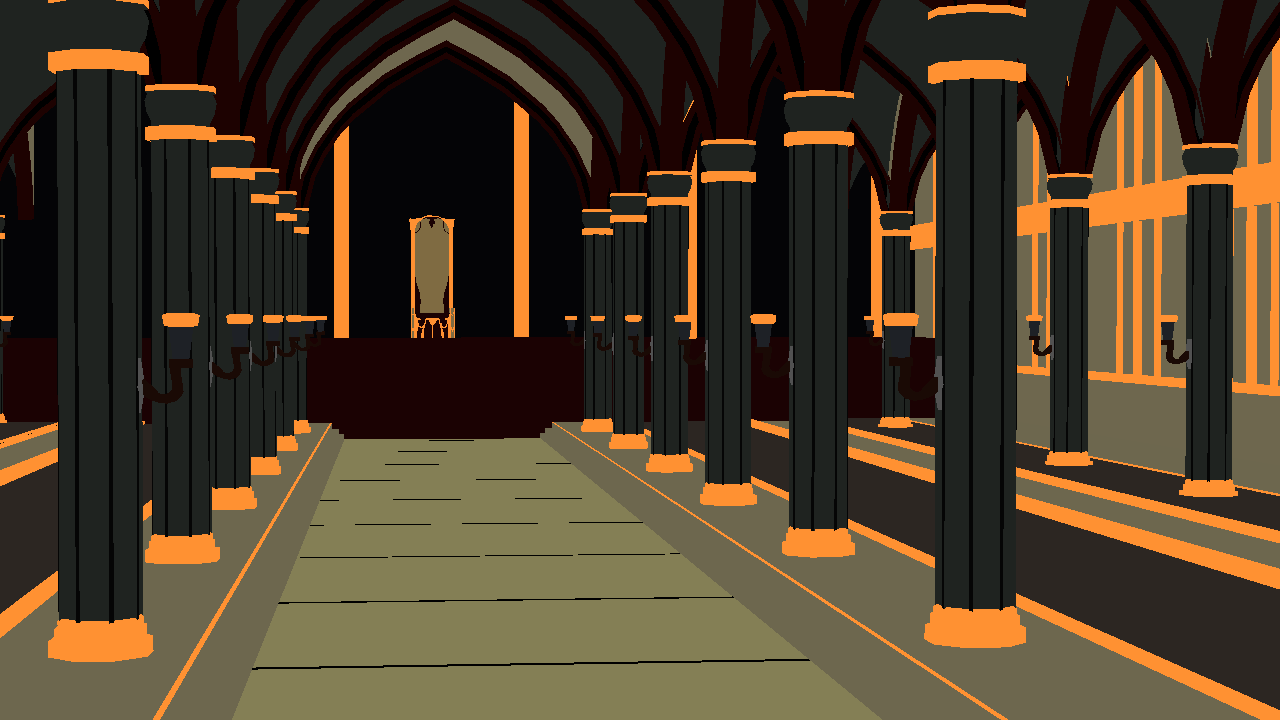
\includegraphics[width=\textwidth]{figures/methods/dataset_example/albedo.png}
         \caption{}
         \label{fig:rendering_dataset_albedo}
    \end{subfigure}
    \hfill
    \begin{subfigure}{0.24\linewidth}
        \centering
         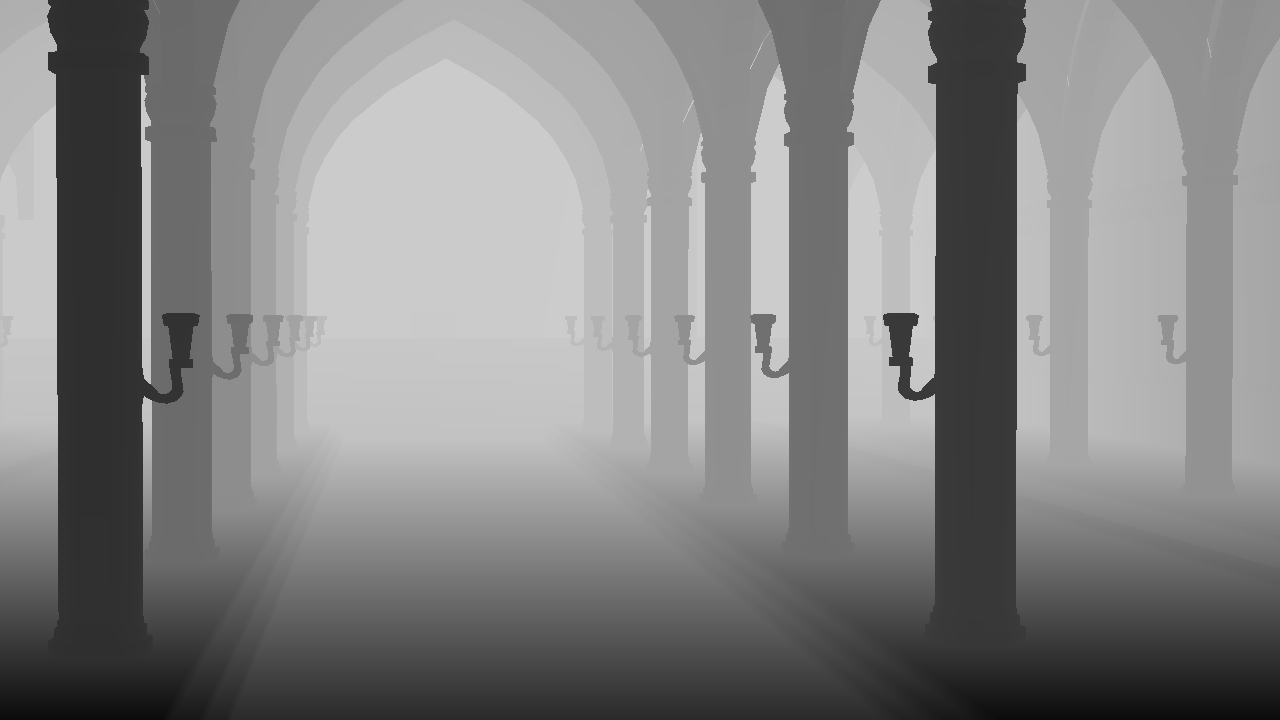
\includegraphics[width=\textwidth]{figures/methods/dataset_example/depth.png}
         \caption{}
         \label{fig:rendering_dataset_depth}
    \end{subfigure}
    \hfill
    \begin{subfigure}{0.24\linewidth}
        \centering
         
\includegraphics[width=\textwidth]{figures/methods/dataset_example/emissive.png}
         \caption{}
         \label{fig:rendering_dataset_emissive}
    \end{subfigure}
    \hfill
    \begin{subfigure}{0.24\linewidth}
        \centering
         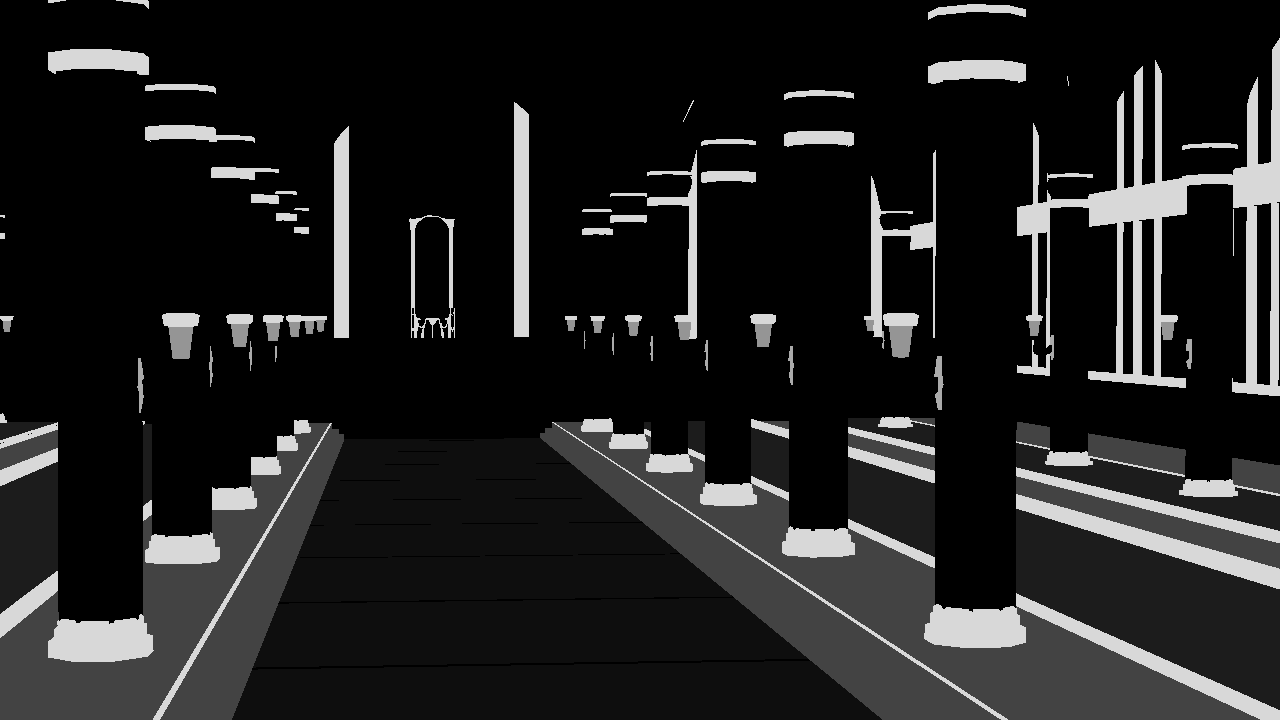
\includegraphics[width=\textwidth]{figures/methods/dataset_example/metallic.png}
         \caption{}
         \label{fig:rendering_dataset_metallic}
    \end{subfigure}
    \\
    \hfill
    \begin{subfigure}{0.24\linewidth}
        \centering
         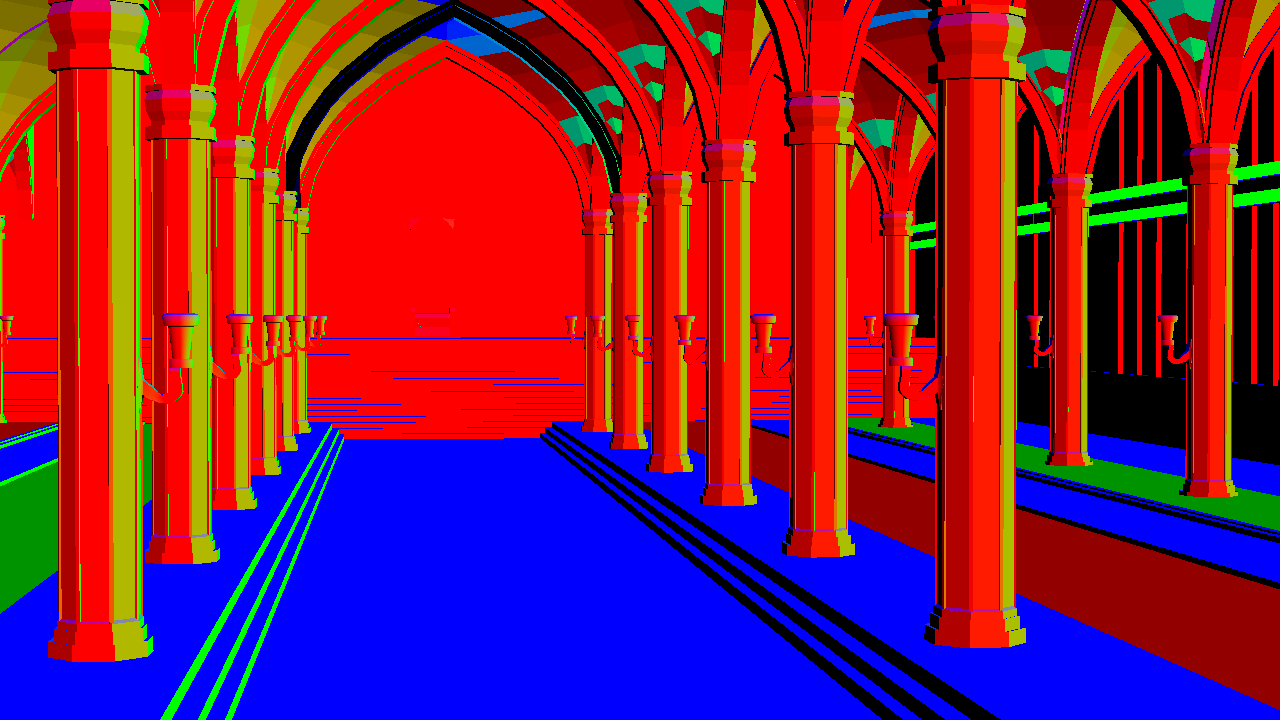
\includegraphics[width=\textwidth]{figures/methods/dataset_example/normal.png}
         \caption{}
         \label{fig:rendering_dataset_normal}
    \end{subfigure}
    \hfill
    \begin{subfigure}{0.24\linewidth}
        \centering
         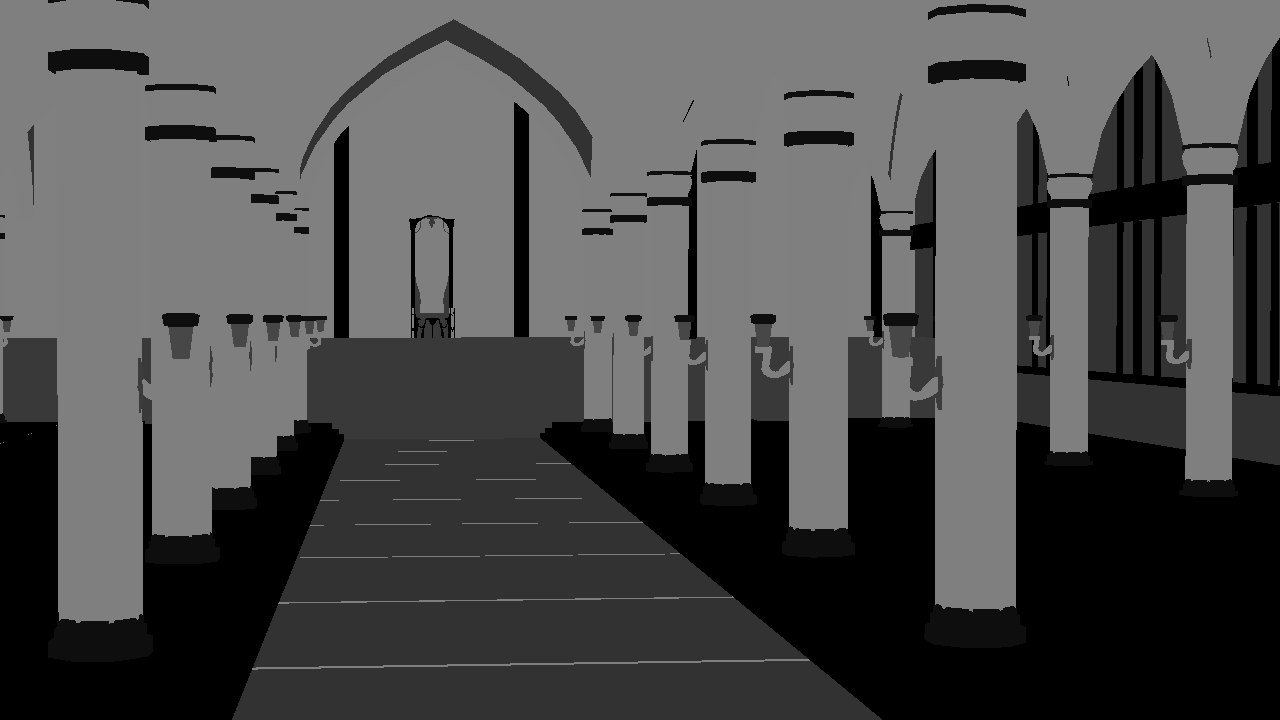
\includegraphics[width=\textwidth]{figures/methods/dataset_example/roughness.png}
         \caption{}
         \label{fig:rendering_dataset_roughness}
    \end{subfigure}
    \hfill
    \begin{subfigure}{0.24\linewidth}
        \centering
         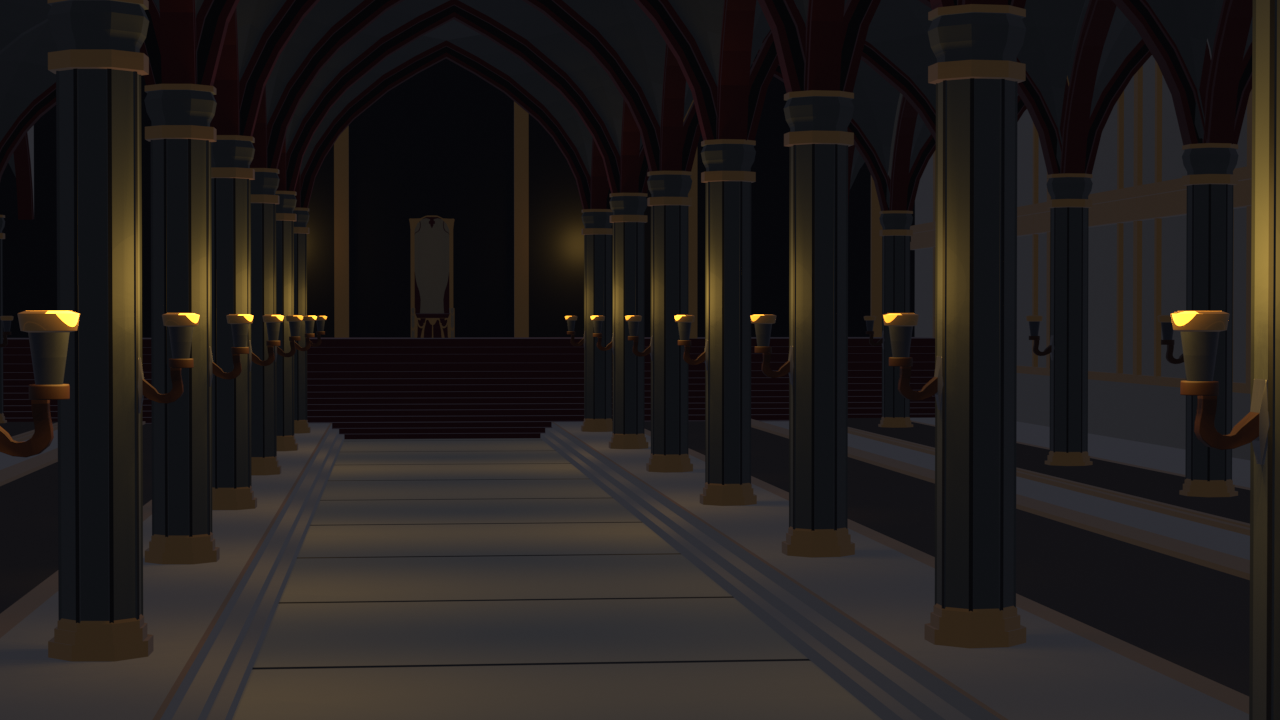
\includegraphics[width=\textwidth]{figures/methods/dataset_example/eevee.png}
         \caption{}
         \label{fig:rendering_dataset_eevee}
    \end{subfigure}
    \hfill
    \begin{subfigure}{0.24\linewidth}
        \centering
         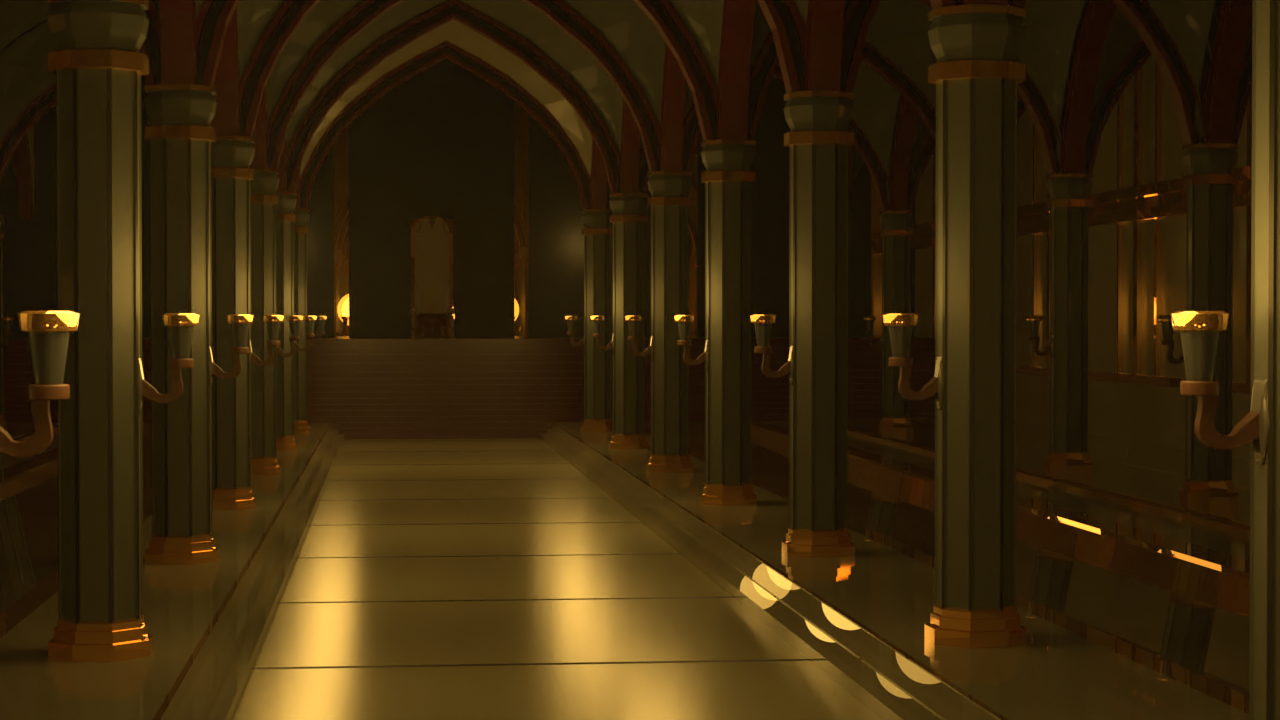
\includegraphics[width=\textwidth]{figures/methods/dataset_example/cycles.png}
         \caption{}
         \label{fig:rendering_dataset_cycles}
    \end{subfigure}
    \caption[Extraction from the RenderDataset]{Examples of the Rendering Dataset. Figure~\ref{fig:rendering_dataset_albedo} showcases an example of albedo data, while Figure~\ref{fig:rendering_dataset_depth} displays an example of the depth map. Figure~\ref{fig:rendering_dataset_emissive} provides an example of the emissive information, and Figure~\ref{fig:rendering_dataset_metallic} presents an example of the metallicness information. Furthermore, Figure~\ref{fig:rendering_dataset_normal} exhibits an example of the surface normal information. The roughness information is displayed in Figure~\ref{fig:rendering_dataset_roughness}, and Figure~\ref{fig:rendering_dataset_eevee} showcases an example of rendering using the real_time rendering engine EEVEE. Lastly, Figure~\ref{fig:rendering_dataset_cycles} offers an example of rendering using the Path_Tracing render engine called Cycles.}
    \label{fig:render_dataset_examples}
    
\end{figure}

\begin{table}[h!]
    \centering
    \begin{tabular}{|c||c|c|c|}
    \toprule
        \multicolumn{3}{|c||}{\textbf{12 scene in total}} & \multicolumn{1}{|c|}{\textbf{Scene}} & \multicolumn{1}{|c|}{\textbf{\thead{Train}}} & \multicolumn{1}{|c|}{\textbf{Test}} & \multicolumn{1}{|c|}{\textbf{Total per scene}}\\
    \midrule
        $1$ & $70$ & $22$ & $92$\\
        $2$ & $82$ & $20$ & $102$\\
        $3$ & $74$ & $21$ & $95$\\
        $4$ & $54$ & $20$ & $74$\\
        $5$ & $52$ & $20$ & $72$\\
        $6$ & $177$ & $19$ & $196$\\
        $7$ & $87$ & $19$ & $106$\\
        $8$ & $10$ & $14$ & $24$\\
        $9$ & $73$ & $14$ & $87$\\
        $10$ & $121$ & $13$ & $134$\\
        $11$ & $139$ & $20$ & $159$\\
        $12$ & $96$ & $24$ & $120$\\
    \midrule
        \textbf{Total} & $1035$ & $207$ & $1242$\\
    \bottomrule
    \end{tabular}
    \caption{Dataset description}
    \label{tab:render_dataset_description}
\end{table}

\begin{figure}
    \centering
    \begin{subfigure}{\textwidth}
        \centering
         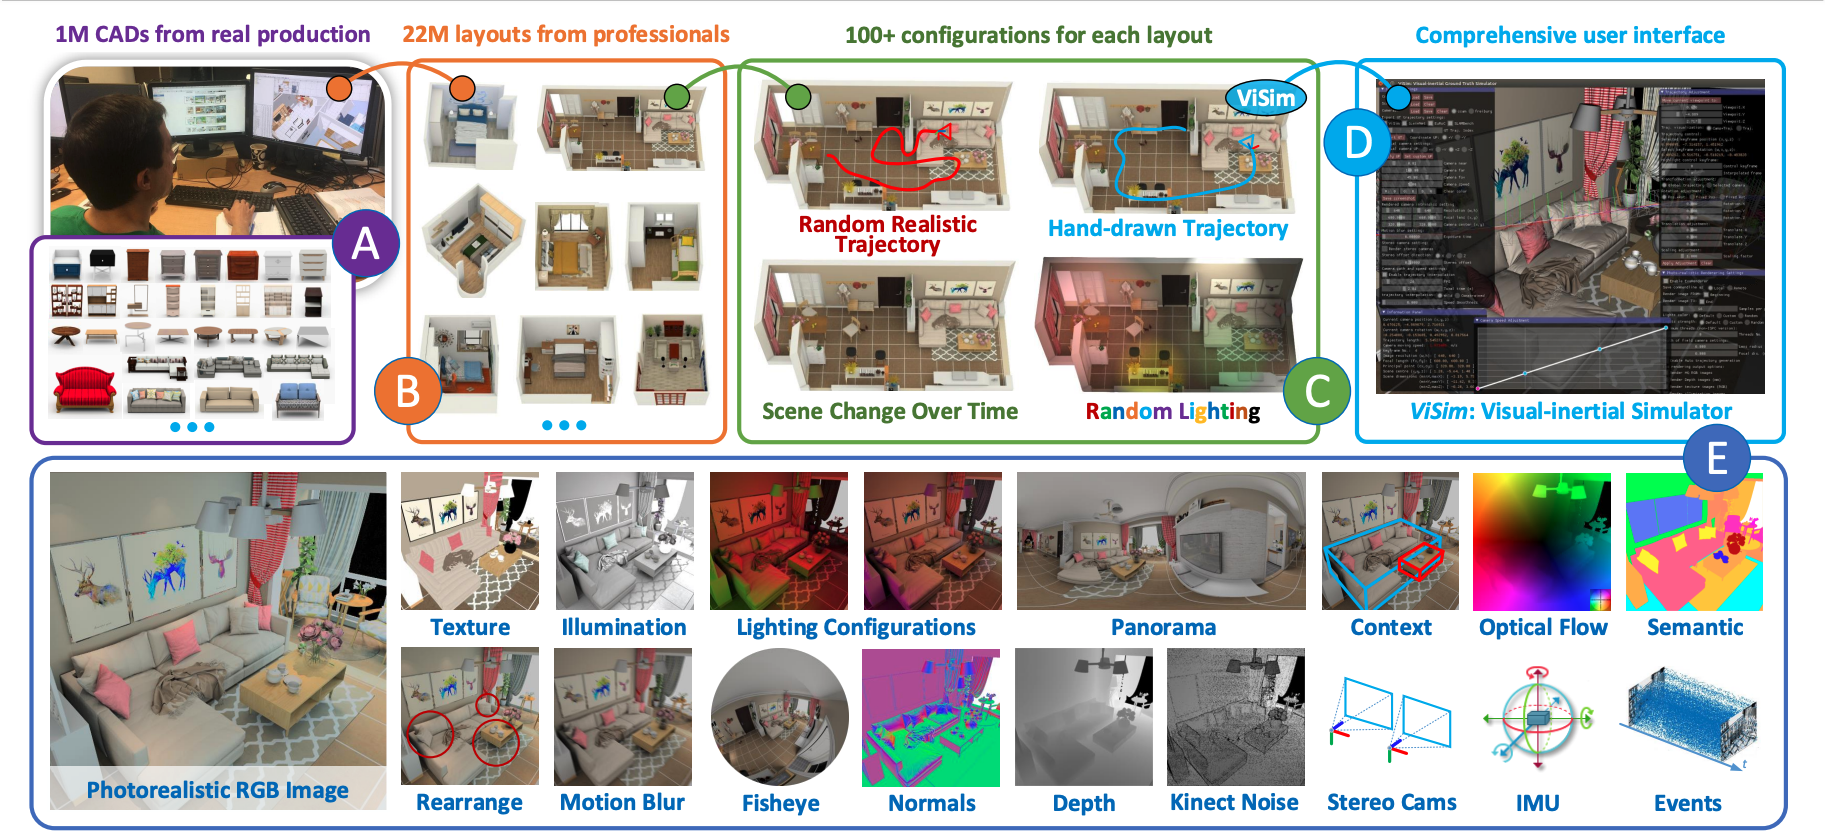
\includegraphics[width=0.75\textwidth]{figures/methods/interiornet.png}
         \caption{}
         \label{fig:rendering_dataset_interiornet}
    \end{subfigure}
    \hfill
    \begin{subfigure}{\textwidth}
        \centering
         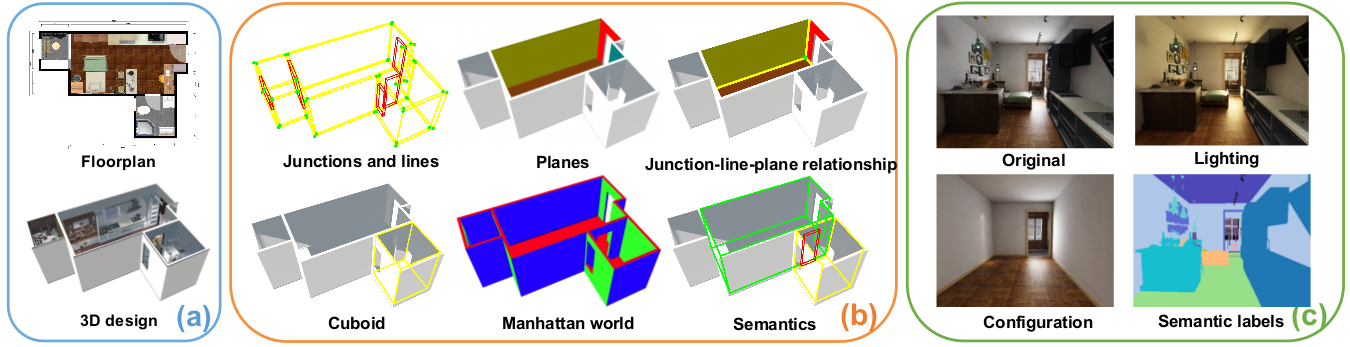
\includegraphics[width=0.75\textwidth]{figures/methods/structured3d.png}
         \caption{}
         \label{fig:rendering_dataset_structured}
    \end{subfigure}
    \caption[State of the Art Dataset for 3D data]{
Illustration of other datasets that lack essential information required for the intended task. These datasets do not provide all the necessary data elements for the completion of the task at hand.}
    \label{fig:render_dataset_other_example}
\end{figure}

\begin{figure}[!h]
\centering
    \begin{subfigure}{0.45\linewidth}
        \centering
         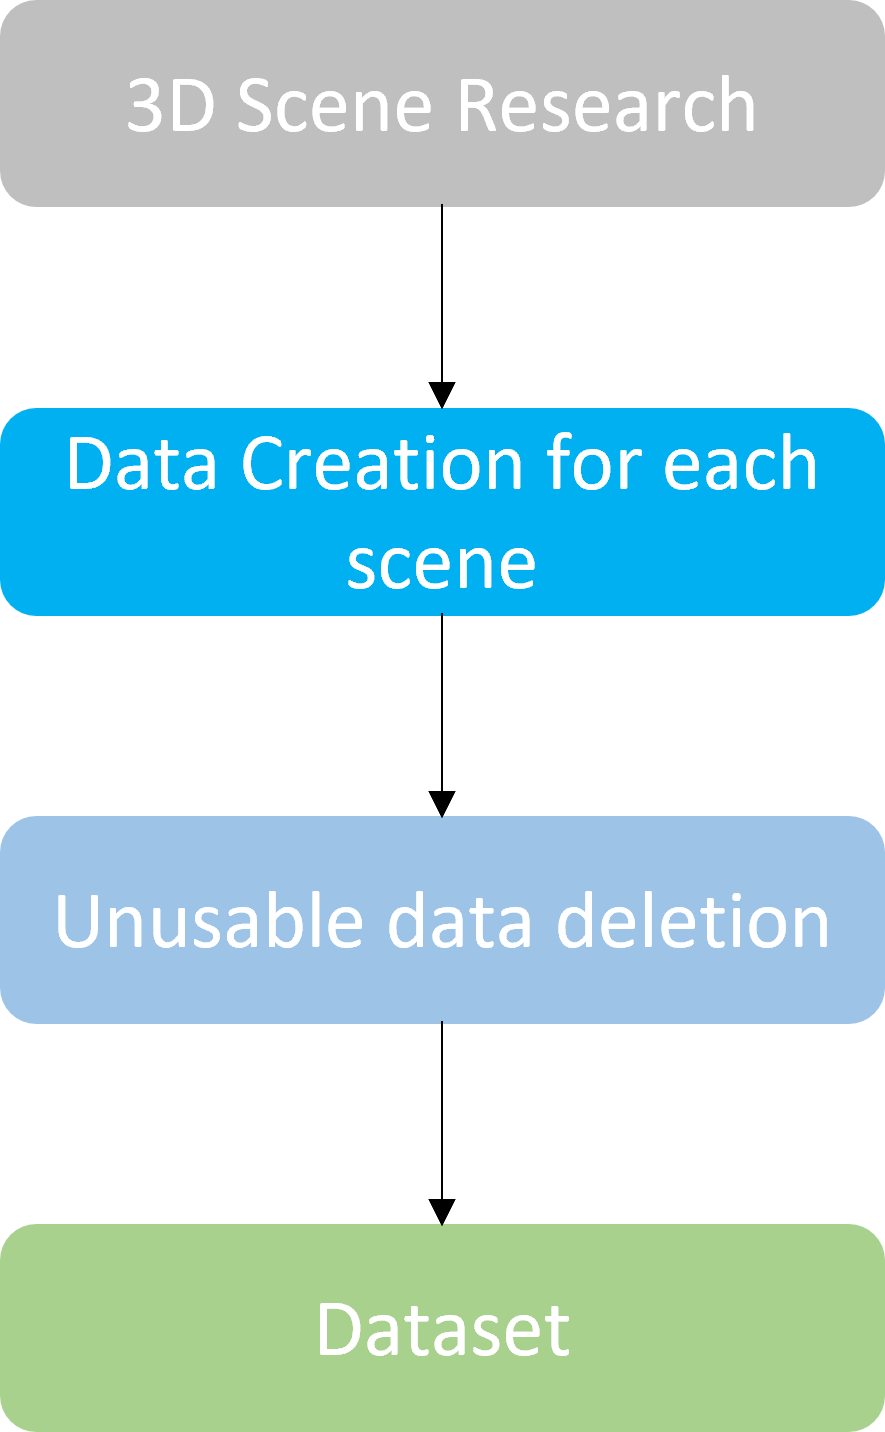
\includegraphics[width=0.45\textwidth]{figures/methods/WorkflowGeneraleCreazioneDataset.png}
         \caption{}
         \label{fig:rendering_dataset_generation_complete}
    \end{subfigure}
    \hfill
    \begin{subfigure}{0.45\linewidth}
        \centering
         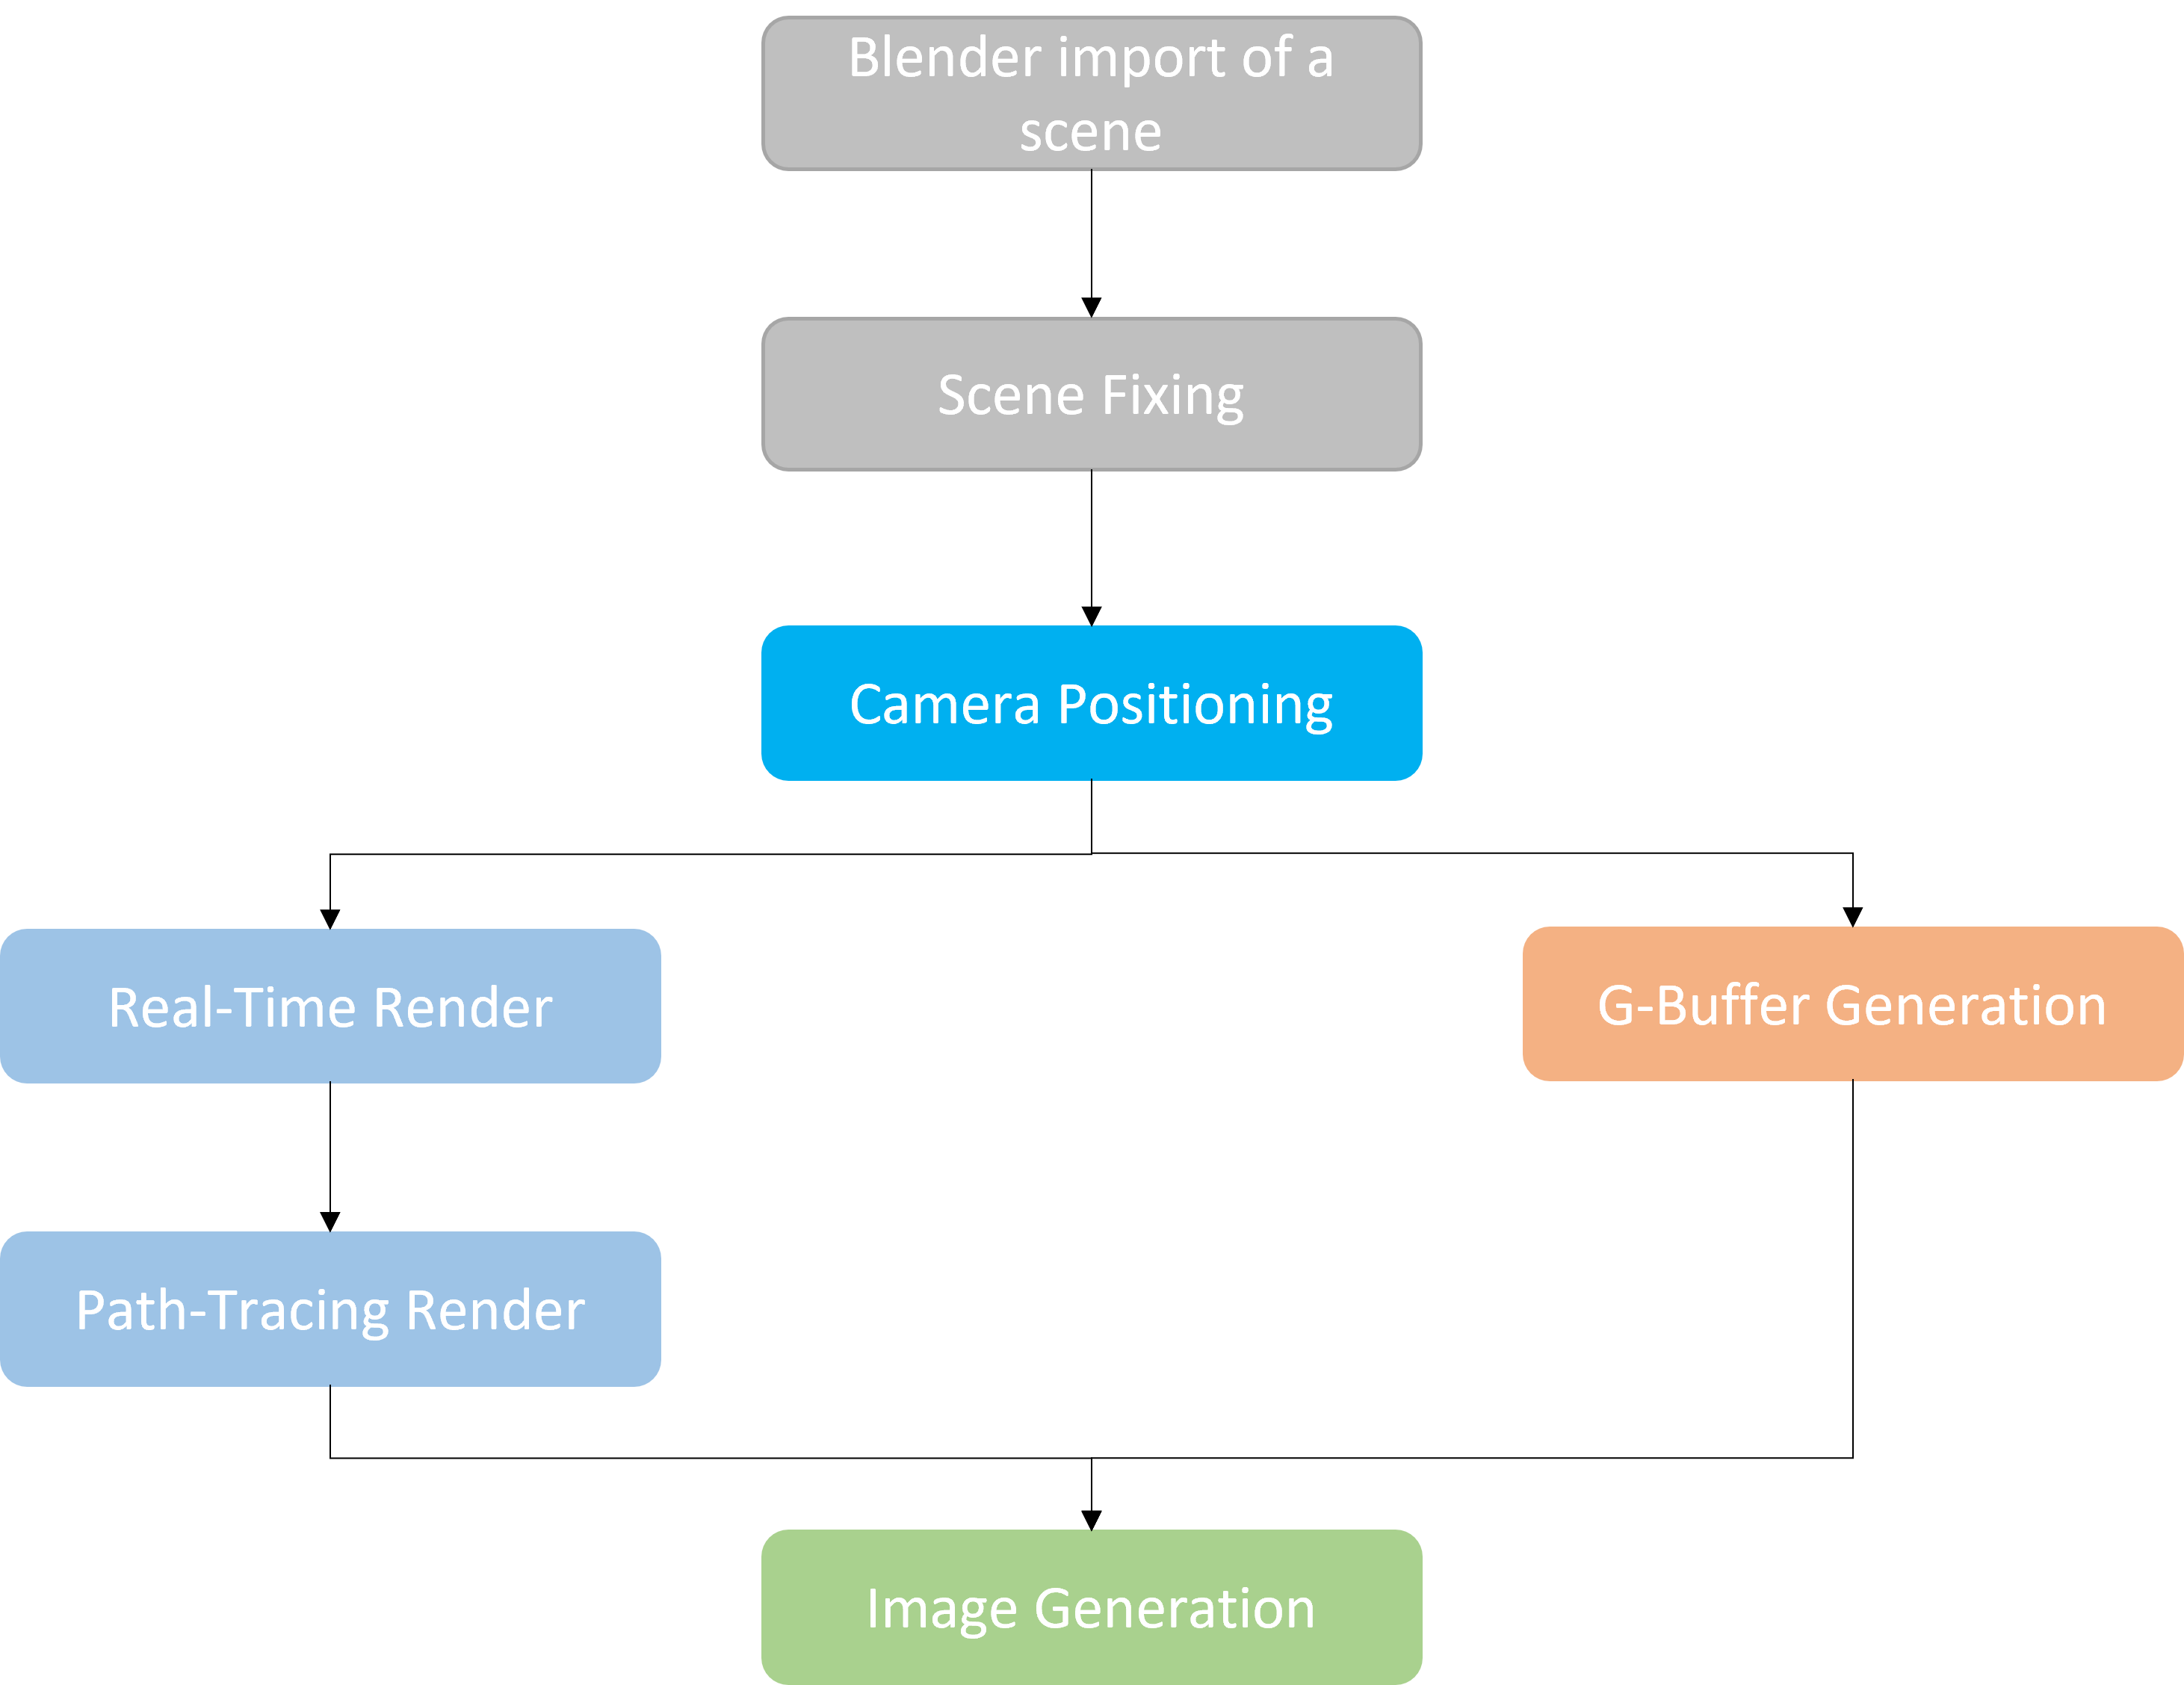
\includegraphics[width=\textwidth]{figures/methods/WorkflowGenerazioneImmaginiBlender.png}
         \caption{}
         \label{fig:rendering_dataset_generation_image}
    \end{subfigure}
\caption[Workflow RenderDataset generalization]{Workflow for the RenderDataset generation. Figure~\ref{fig:rendering_dataset_generation_image} presents a detailed view of the image generation process, which serves as an expansion of the second block depicted in Figure~\ref{fig:rendering_dataset_generation_complete}.}
\label{fig:render_dataset_generation}
\end{figure}

The 3D scenes were obtained from Sketchfab~\footnote{https://sketchfab.com/} and imported into Blender, where necessary adjustments were made to ensure their suitability for the intended purpose. Multiple cameras were strategically positioned to capture various views of each scene. Subsequently, the scenes were rendered using both the real_time engine and the path_tracing engine. Additionally, G_Buffers were computed simultaneously, storing all relevant information in image format and organizing it into a structured dataset as depicted in Figure~\ref{fig:render_dataset_structure}.

\begin{figure}
    \centering
    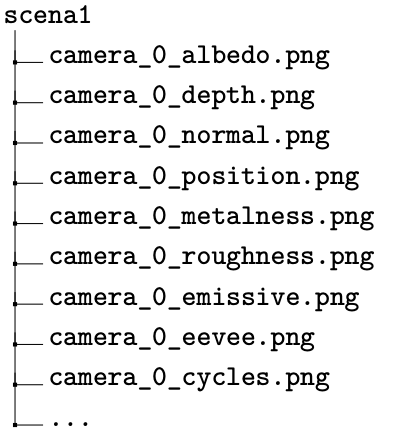
\includegraphics[width=0.45\textwidth]{figures/methods/StrutturaCartellaDataset.png}
    \caption{Example of the structure of the dataset in the folder}
    \label{fig:render_dataset_structure}
\end{figure}

During the image selection process, a careful examination of the rendered images enables the identification of distinct characteristics that distinguish the outputs of the EEVEE and Cycles render engines. Several examples highlighting these differences are showcased in Figure~\ref{fig:rendering_dataset_diff_riflessi_cycles} and Figure~\ref{fig:rendering_dataset_piccole_cycles} and Figure~\ref{fig:rendering_dataset_grandi_cycles} and Figure~\ref{fig:rendering_dataset_grandi_eevee} clearly exhibit the stark contrast in the rendering result, with Cycles providing more accurate and realistic volume and shadow arrangements, while EEVEE produces flatter and less refined images, resembling sketches rather than renders.

\begin{figure}
    \centering
    \begin{subfigure}{0.24\linewidth}
        \centering
         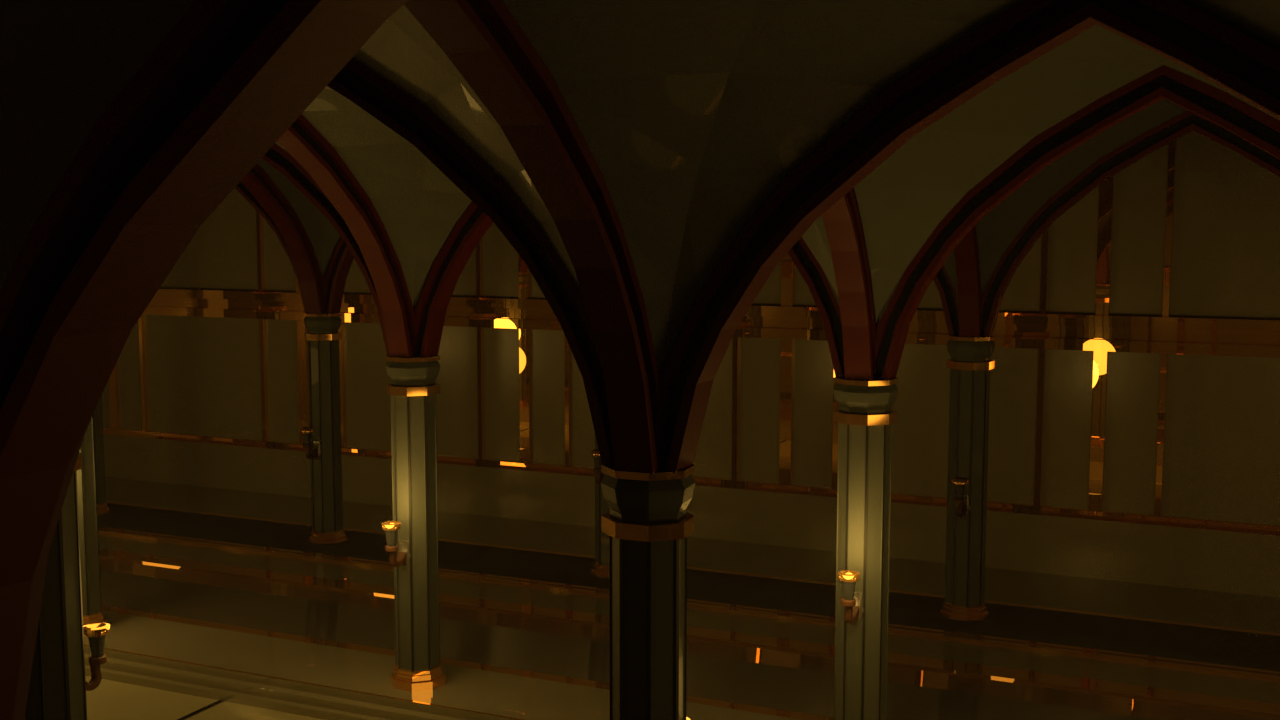
\includegraphics[width=\textwidth]{figures/methods/dataset_compare/diff_riflessi_cycles.png}
         \caption{}
         \label{fig:rendering_dataset_diff_riflessi_cycles}
    \end{subfigure}
    \hfill
    \begin{subfigure}{0.24\linewidth}
        \centering
         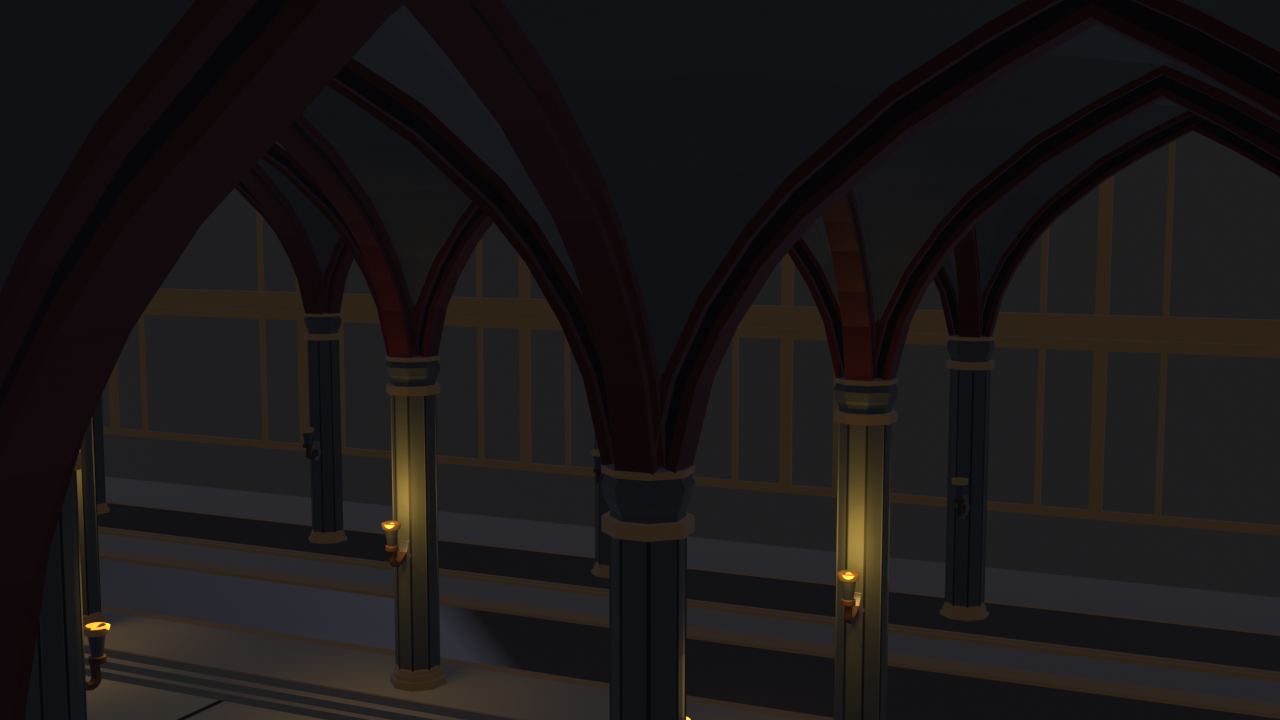
\includegraphics[width=\textwidth]{figures/methods/dataset_compare/diff_riflessi_eevee.png}
         \caption{}
         \label{fig:rendering_dataset_diff_riflessi_eevee}
    \end{subfigure}
    \hfill
    \begin{subfigure}{0.24\linewidth}
        \centering
         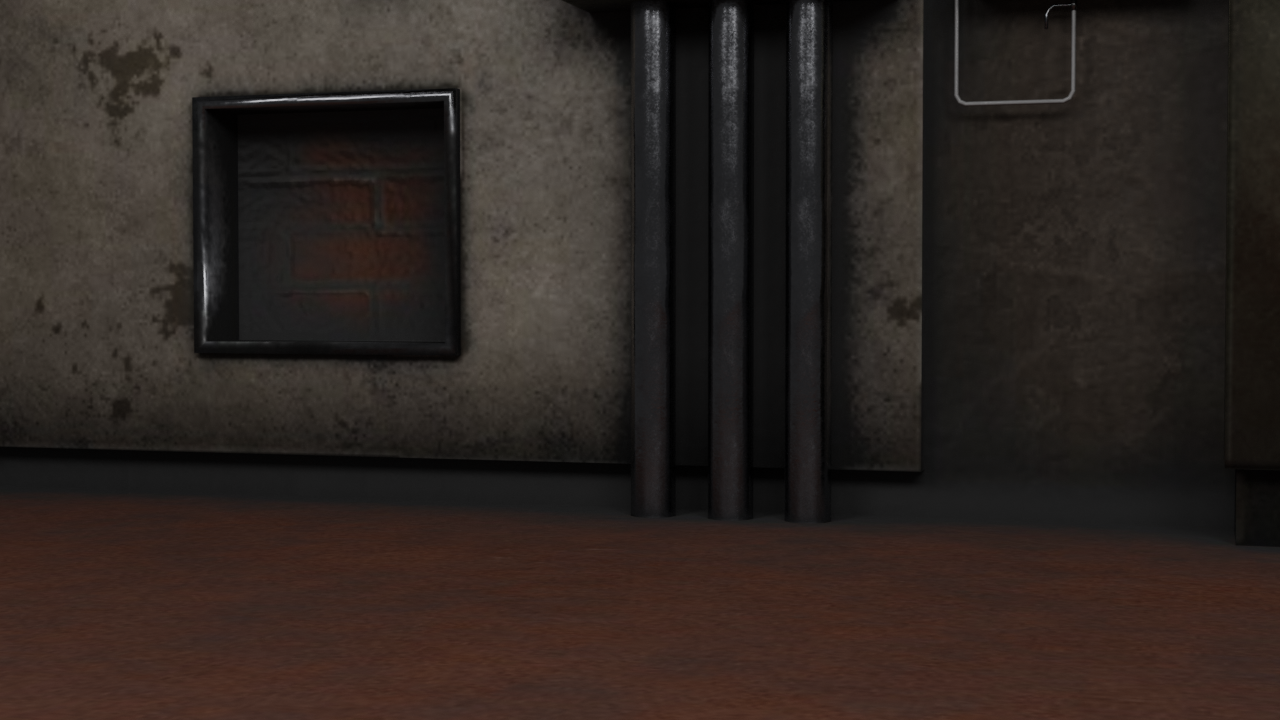
\includegraphics[width=\textwidth]{figures/methods/dataset_compare/piccole_differenze_cycles.png}
         \caption{}
         \label{fig:rendering_dataset_piccole_cycles}
    \end{subfigure}
    \hfill
    \begin{subfigure}{0.24\linewidth}
        \centering
         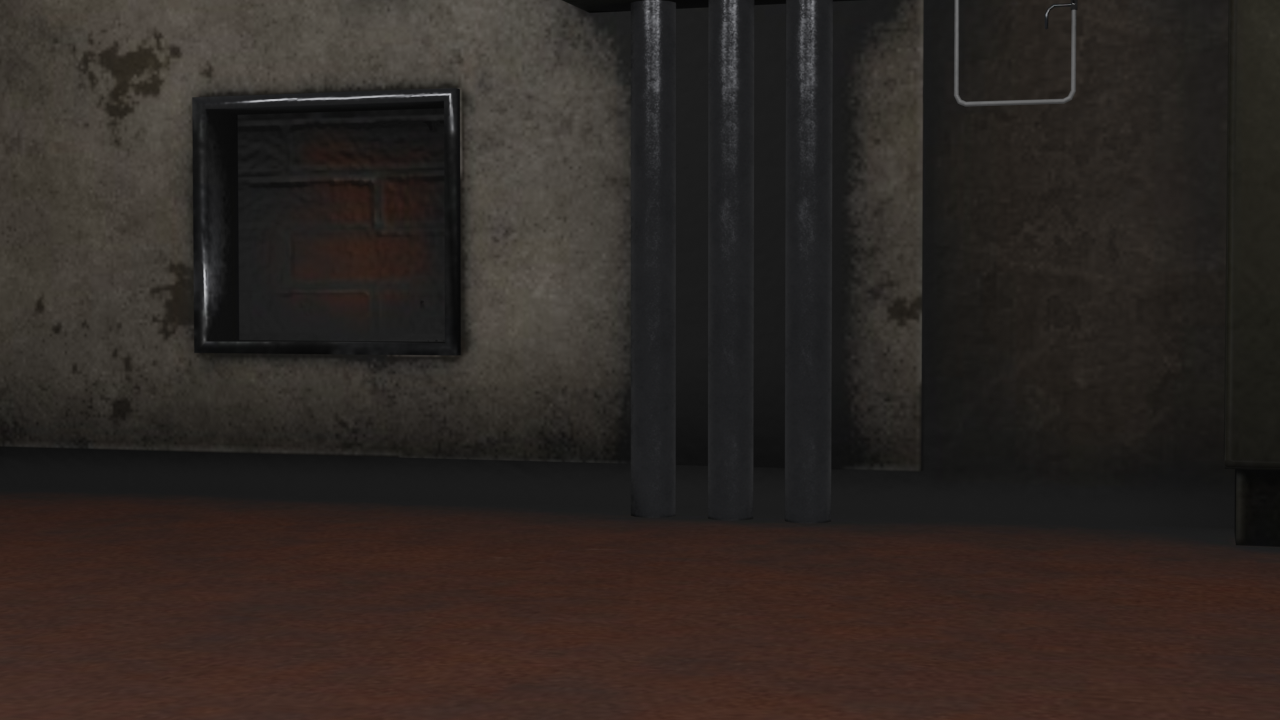
\includegraphics[width=\textwidth]{figures/methods/dataset_compare/piccole_differenze_eevee.png}
         \caption{}
         \label{fig:rendering_dataset_piccole_eevee}
    \end{subfigure}
    \hfill
    \begin{subfigure}{0.24\linewidth}
        \centering
         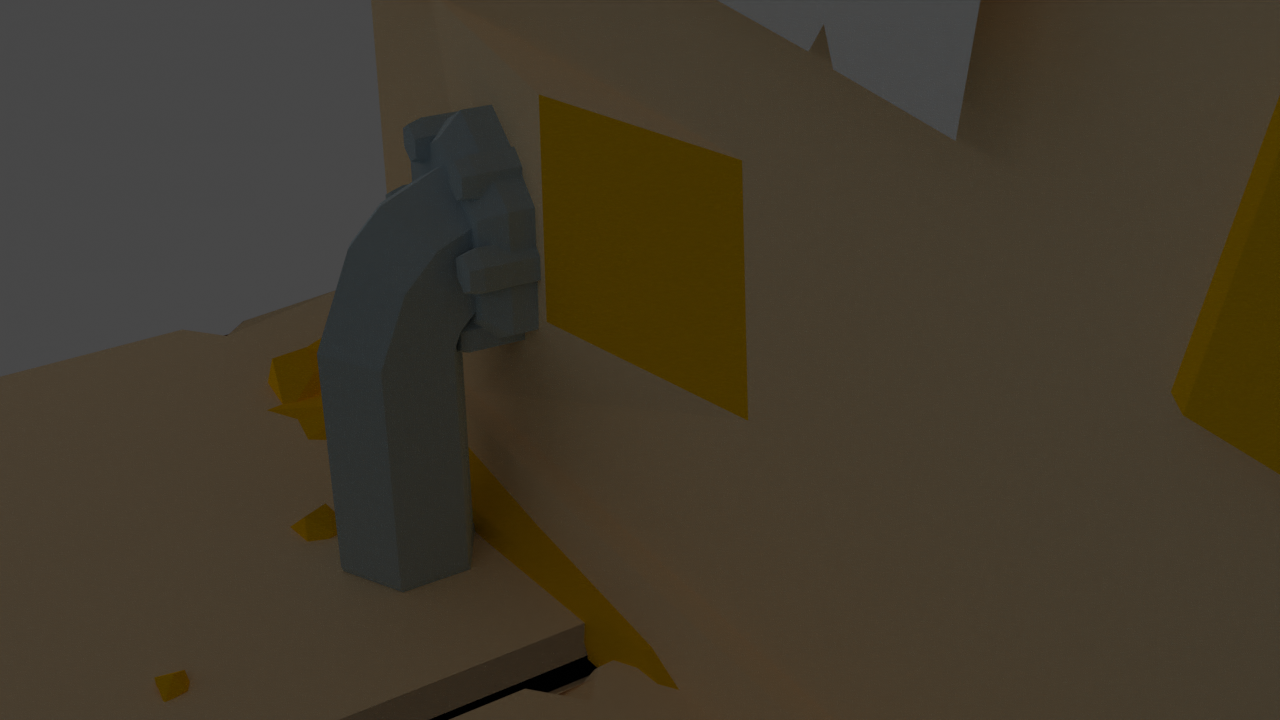
\includegraphics[width=\textwidth]{figures/methods/dataset_compare/grandi_diff_cycles.png}
         \caption{}
         \label{fig:rendering_dataset_grandi_cycles}
    \end{subfigure}
    \hfill
    \begin{subfigure}{0.24\linewidth}
        \centering
         
\includegraphics[width=\textwidth]{figures/methods/dataset_compare/grandi_diff_eevee.png}
         \caption{}
         \label{fig:rendering_dataset_grandi_eevee}
    \end{subfigure}
    \caption[Rendering result based on the bitmap engine EEVEE]{Example of the rendering result. On the left are the cycles rendering result, and on the right, there is the Eevee rendering result.}
    \label{fig:render_dataset_comparison}
\end{figure}

\subsection{Network Configuration}
The primary objective of our network is to discover a function that can generate rendered images perceptually similar to those produced by the Cycles engine, given input from the EEVEE image and information from the G_Buffer. To achieve this, it is crucial to consider how the algorithm interprets perception.

\subsubsection{Perceptual Loss}
Perceptual loss is a critical component of the overall loss function, driving the network to produce natural and visually pleasing result. Previous studies \cite{zhao2017loss, ding2021comparison} have explored various loss functions, including $L1$, $L2$, Structural Similarity Index ($SSIM$), and MultiScale_Structural Similarity Index ($MS_SSIM$), to measure image quality in super_resolution algorithms. However, classical metrics like $L1$ tend to produce sharpened images, disregarding the varying importance of different regions in the image. To address this issue, we adopt the perceptual loss function proposed by Johnson et al. \cite{johnson2016perceptual}.

The perceptual loss leverages a \textbf{Loss Network}, based on the VGG16 convolutional network architecture \cite{simonyan2014very}, which is pre_trained on ImageNet \cite{imagenet2009dataset}. The Loss Network extracts content and style information from both the reference (Cycles_rendered) and generated images. Specifically:
\begin{itemize}
\item Content information is extracted from the '\textit{$relu3_3$}' layer of the generated image.
\item The reference representation is extracted from the '\textit{$relu1_2$}', '\textit{$relu2_2$}', '\textit{$relu3_3$}', and '\textit{$relu4_3$}' layers of the reference image (rendered using the Cycles engine).
\end{itemize}

The extracted representations are utilized to compute two types of loss:

\subsubsection{Feature Reconstruction Loss}
The feature reconstruction loss is calculated using the output image, i.e., the image generated by the generator, and extracting its representation from the '\textit{$relu3_3$}' layer. The loss function is defined as follows:
\begin{equation}
l_{feat}^{\Phi,J} (\hat{y}, y) = \frac{1}{C_J * H_J * W_J} ||\Phi_J(\hat{y}) _ \Phi_J(y)||_2^2
\label{eq:render_feature_reconstruction_loss}
\end{equation}

\subsubsection{Style Reconstruction Loss}
The style reconstruction loss is calculated using the generated image and the style reference obtained from the '\textit{$relu1_2$}', '\textit{$relu2_2$}', '\textit{$relu3_3$}', and '\textit{$relu4_3$}' layers of the Loss Network:
\begin{equation}
l_{style}^{\Phi,J} = || G_J^{\Phi} (\hat{y}) _ G_J^{\Phi}(y)||_F^2 ||
\label{eq:render_style_reconstruction_loss}
\end{equation}

The total loss is typically the weighted sum of Equation\ref{eq:render_style_reconstruction_loss}.

The network architecture used for rendering image generation combines the Encoder_Decoder approach with the GAN framework. The network consists of seven encoders based on the EfficientNet \cite{tan2019efficientnet}, which extract features from the input images (EEVEE and G_Buffers). These extracted features are then concatenated and used as input for the decoder, which employs transposed convolution for image generation.

\subsection{Transposed Convolution Issues}
Transposed convolution, also known as Upsampled Convolution, allows upsampling of input feature maps. It overcomes some of the limitations of other upsampling methods such as Nearest Neighbors, Bi_Linear Interpolation, Bed of Neils, and Max Pooling.

The transposed convolution follows a specific workflow:
\begin{enumerate}
\item An input with a size of, for example, 2x2, needs to be upsampled to a desired output size, e.g., 3x3.
\item A kernel of size 2x2 with unit stride and zero padding is applied to the input.
\item The upper left element of the input is multiplied with every element of the kernel, and this process is repeated for all remaining input elements, resulting in four different 2x2 matrices, each corresponding to an input element's position.
\item Some elements of the resulting upsampled matrices may overlap, causing issues in the output. To address this, the elements of overlapping regions are added together to eliminate artifacts.
\item The final output is obtained, producing the upsampled matrix with the required spatial dimensions, in this case, 3x3.
\end{enumerate}

However, transposed convolution can introduce undesirable patterns in the output, as shown in Figure~\ref{fig:render_trasposed_convolution_pattern_problem}. This problem arises when the image has sections that are not perfectly superimposable with each other.

To address this issue, previous studies \cite{gauthier2014conditional, odena2016deconvolution} proposed various solutions, including using non_divisible kernel sizes for the stride and employing the nearest neighbor approach followed by convolution. In our approach, we combine the strengths of these methods by using transposed convolution layers in conjunction with convolution layers to eliminate patterns. Specifically, we apply normal convolution with a kernel size equal to 1, which leaves the feature size unchanged. This creates a projection of the image obtained through transposed convolution onto a continuous space, preserving all information while eliminating undesirable patterns. The modified approach also establishes connections between various extracted data, ensuring a cohesive link between different input sources. This solution employs transposed convolution layers with convolution layers to eliminate patterns. Specifically, we use normal convolution with a kernel size equal to 1, leaving the feature size unchanged. This creates a projection of the image obtained through transposed convolution onto a continuous space, preserving all information while eliminating undesirable patterns. The modified approach establishes connections between various extracted data, ensuring a cohesive link between different input sources. By leveraging this hybrid approach, we mitigate the issues associated with transposed convolution and improve the overall quality of the rendered images. The resulting network architecture effectively addresses perceptual loss and transposed convolution problems, allowing us to generate visually appealing and realistic images closely resembling those produced by the Cycles engine. Figures~\ref{fig:render_network_configuration} and~\ref{fig:render_trasposed_convolution_pattern_problem} illustrate the network configuration and the transposed convolution pattern problem, respectively, providing a comprehensive understanding of our approach's architecture and challenges.

\subsection{Image Quality Evaluation Indices}
In order to assess the performance and improvement of RenderGAN, a comprehensive image quality evaluation is essential. For this purpose, we employ two prominent indices: the Structural Similarity Index Measure (SSIM) and the Universal Image Quality Index (UIQI). These metrics offer valuable insights into the similarity and distortion between the generated images and the reference images. The SSIM utilizes a multi_scale approach, measuring image similarity across different scales, while the UIQI models image distortion by considering the loss of correlation, luminance distortion, and contrast distortion relative to the reference image. 

\subsubsection{Structural Similarity Index Measure (SSIM)}

The Structural Similarity Index Measure (SSIM) is employed in this study to evaluate the similarity between two images. SSIM, as defined in \cite{wang2003multiscale}, incorporates the concept of Multi_Scale SSIM, which applies SSIM on M scales, with scale 1 representing the input image. The SSIM index measures the structural similarity between the generated images and the ground truth. It is defined by the following equation:

\begin{equation}
    \text{SSIM}(f, g) = \frac{(2\mu_{f}\mu_{g} + C_1)(2\sigma_{fg} + C_2)}{(\mu_{f}^2 + \mu_{g}^2 + C_1)(\sigma_{f}^2 + \sigma_{g}^2 + C_2)}
\end{equation}

where:
_ $\mu_{f}$ and $\mu_{g}$ are the means of images $f$ and $g$ respectively.
_ $\sigma_{f}$ and $\sigma_{g}$ are the standard deviations of images $f$ and $g$ respectively.
_ $\sigma_{fg}$ is the covariance of images $f$ and $g$.
_ $C_1$ and $C_2$ are constants to stabilize the division, typically $C_1 = (k_1L)^2$ and $C_2 = (k_2L)^2$ where $L$ is the dynamic range of pixel values and $k_1$ and $k_2$ are constants.

The SSIM index ranges from _1 to 1, where a value of 1 indicates perfect similarity, a value close to _1 suggests strong dissimilarity, and 0 indicates no correlation between the images.

\subsubsection{Universal Image Quality Index (UIQI)}
The Universal Image Quality Index (UIQI) is another metric employed in this study, and its equations are provided in \cite{universal_image_quality_index}. The UIQI mathematically defines image distortion relative to a reference image by considering three factors: loss of correlation, luminance distortion, and contrast distortion. For two images $f$ and $g$, represented as matrices with $M$ columns and $N$ rows containing pixel values $f[i,j]$ and $g[i,j]$ respectively $(0 \geq i > M, 0 \geq j > N)$, the UIQI $Q$ is calculated as a product of three components:

\begin{equation}
    Q = \frac{\sigma_{fg}}{\sigma_{f}\sigma_{g}} \times \frac{2\mu_{f}\mu_{g}}{\mu_{f}^2 + \mu_{g}^2 + C_1} \times \frac{2\sigma_{f}\sigma_{g}}{\sigma_{f}^2 + \sigma_{g}^2 + C_2}
\end{equation}

where:
\begin{itemize}
    \item The first component represents the correlation coefficient, which measures the degree of linear correlation between images $f$ and $g$. It varies in the range [_1, 1], and the best value of 1 is obtained when $f$ and $g$ are linearly related, meaning $g[i,j] = af[i,j] + b$ for all possible values of $i$ and $j$.
    \item The second component measures how close the mean luminance is between images $f$ and $g$.
    \item The third component measures how similar the contrasts of the images are.
\end{itemize}

The trend of these metrics is analyzed to assess the progressive improvement in the quality of the network_generated images throughout the training process.

\section{result and Discussions}
\label{sec:rendering_result}
In this section, we present the result obtained from our rendering approach, which was evaluated using a 40GB A100 and trained for 500 epochs. The RMSProp optimizer, recommended in the Wasserstein GAN framework, was utilized to optimize the network's performance. To gauge the progress of the training process, we monitored the loss trends of both the discriminator and the generator. As expected, the discriminator loss demonstrated a decreasing trend, reaching a final value of 0.000146, indicating that the discriminator effectively learned to distinguish between real and generated images. On the other hand, the generator's L1 distance steadily decreased to a value of 0.009841, signifying the consistent improvement of the generator's output over the training period. Furthermore, the perceptual loss, an important component of our network's overall loss function, exhibited a declining trend, reaching a minimum value of $0.09785$. Additionally, the graphs revealed that the generator was trained every three updates of the discriminator, ensuring a balanced and effective training process. These result provide valuable insights into the effectiveness of our rendering approach, demonstrating the network's ability to produce high_quality and visually realistic images. 

\subsubsection{Ablation study}

To verify that the result obtained need all input data, an ablation Study was applied to the convolutional layers of the encoder to understand which data are beneficial. Data were used individually as well as in combination.

\begin{table}[h!t]
    \centering
    \begin{tabular}{|r||c|c|c|c|c|}
    \toprule
        \multicolumn{1}{|c||}{\textbf{EEVEE}} & \multicolumn{1}{|c|}{\textbf{L1}} & \multicolumn{1}{|c|}{\textbf{\thead{Perceptual\\ Loss}}} & \multicolumn{1}{|c|}{\textbf{SSIM}} & \multicolumn{1}{|c|}{\textbf{MSSIM}} & \multicolumn{1}{|c|}{\textbf{UIQI}} \\
    \midrule
        Albedo & $0,303$ & $1,51$ & $0,695$ & $0,586$ & $0,00087$ \\
        Depth & $0,235$ & $1,62$ & $0,699$ & $0,794$ & $0,003$ \\
        Normal & $0,323$ & $1,68$ & $0,600$ & $0,553$ & $0,00084$ \\
        Emissive & $0,398$ & $1,55$ & $0,719$ & $0,689$ & $0,00011$ \\
        Metalness & $0,368$ & $2,03$ & $0,776$ & $0,708$ & $0,0025$ \\
        Roughness & $0,368$ & $1,88$ & $0,723$ & $0,653$ & $0,00050$ \\
        Position & $0,262$ & $1,45$ & $0,745$ & $0,591$ & $0,00056$ \\
        \textbf{All} & \textbf{$0,009$} & \textbf{$0,09$} & \textbf{$0,912$} & \textbf{$0,982$} & \textbf{$0,898$} \\
    \bottomrule
    \end{tabular}
    \caption{Result of the RenderGAN network with one additional input}
    \label{tab:render_single_input_table}
\end{table}

\begin{table}[h!]
    \centering
    \begin{adjustbox}{width=\textwidth}
    \begin{tabular}{|r||c|c|c|c|c|}
    \toprule
        \multicolumn{1}{|c||}{\textbf{EEVEE}} & \multicolumn{1}{|c|}{\textbf{L1}} & \multicolumn{1}{|c|}{\textbf{\thead{Perceptual\\ Loss}}} & \multicolumn{1}{|c|}{\textbf{SSIM}} & \multicolumn{1}{|c|}{\textbf{MSSIM}} & \multicolumn{1}{|c|}{\textbf{UIQI}} \\
    \midrule
        \textbf{Depth + Normal} & $0,362$ & $1,62$ & $0,651$ & $0,537$ & $0,002$ \\
        \textbf{Depth + Albedo} & $0,244$ & $1,61$ & $0,661$ & $0,663$ & $0,005$ \\
        \textbf{Depth + Emissive} & $0,432$ & $2,29$ & $0,930$ & $0,826$ & $0,001$ \\
        \textbf{Depth + Metalness} & $0,501$ & $2,20$ & $0,773$ & $0,598$ & $0,0005$ \\
        \textbf{Depth + Roughness} & $0,408$ & $1,51$ & $0,735$ & $0,598$ & $0,0005$ \\
        \textbf{Depth + Position} & $0,392$ & $2,10$ & $0,756$ & $0,671$ & $0,001$ \\
        \textbf{Albedo + Normal} & $0,305$ & $1,57$ & $0,633$ & $0,549$ & $0,001$ \\
        \textbf{Albedo + Emissive} & $0,449$ & $2,53$ & $0,913$ & $0,836$ & $0,0005$ \\
        \textbf{Albedo + Metalness} & $0,409$ & $2,09$ & $0,687$ & $0,637$ & $0,001$ \\
        \textbf{Albedo + Roughness} & $0,398$ & $2,11$ & $0,601$ & $0,605$ & $0,005$ \\
        \textbf{Albedo + Position} & $0,414$ & $2,12$ & $0,664$ & $0,607$ & $0,0001$ \\
        \textbf{Normal + Emissive} & $0,406$ & $1,98$ & $0,883$ & $0,688$ & $0,0003$ \\
        \textbf{Normal + Metalness} & $0,494$ & $2,39$ & $0,661$ & $0,559$ & $0,0003$ \\
        \textbf{Normal + Roughness} & $0,612$ & $2,10$ & $0,624$ & $0,515$ & $0,0004$ \\
        \textbf{Normal + Position} & $0,454$ & $2,15$ & $0,622$ & $0,597$ & $0,0009$ \\
        \textbf{Emissive + Metalness} & $0,349$ & $2,25$ & $0,895$ & $0,775$ & $0,003$ \\
        \textbf{Emissive + Roughness} & $0,283$ & $2,09$ & $0,900$ & $0,837$ & $0,002$ \\
        \textbf{Emissive + Position} & $0,445$ & $1,90$ & $0,922$ & $0,823$ & $0,0008$ \\
        \textbf{Metalness + Roughness} & $0,590$ & $2,29$ & $0,275$ & $0,901$ & $0,0001$ \\
        \textbf{Metalness + Psotion} & $0,443$ & $2,31$ & $0,716$ & $0,649$ & $0,0009$ \\
    \bottomrule
    \end{tabular}
    \end{adjustbox}
    
    \caption{RenderGAN result on double input data}
    \label{tab:render_double_data}
\end{table}

\begin{table}[h!]
    \centering
    \begin{adjustbox}{width=\textwidth}
    \begin{tabular}{|r||c|c|c|c|c|}
    \toprule
        \multicolumn{1}{|c||}{\textbf{EEVEE}} & \multicolumn{1}{|c|}{\textbf{L1}} & \multicolumn{1}{|c|}{\textbf{\thead{Perceptual\\ Loss}}} & \multicolumn{1}{|c|}{\textbf{SSIM}} & \multicolumn{1}{|c|}{\textbf{MSSIM}} & \multicolumn{1}{|c|}{\textbf{UIQI}} \\
    \midrule
        \textbf{Depth + Albedo + Normal} & $0,285$ & $1,71$ & $0,606$ & $0,640$ & $0,004$ \\
        \textbf{Depth + Albedo + Emissive} & $0,220$ & $0,98$ & $0,870$ & $0,736$ & $0,002$ \\
        \textbf{Depth + Albedo + Metalness} & $0,227$ & $1,56$ & $0,715$ & $0,708$ & $0,006$ \\
        \textbf{Depth + Albedo + Roughness} & $0,300$ & $1,23$ & $0,667$ & $0,575$ & $0,001$ \\
        \textbf{Depth + Albedo + Position} & $0,305$ & $1,64$ & $0,692$ & $0,643$ & $0,002$ \\
        \textbf{Albedo + Normal + Metalness} & $0,229$ & $1,36$ & $0,686$ & $0,679$ & $0,007$ \\
        \textbf{Albedo + Normal + Emissive} & $0,289$ & $1,53$ & $0,852$ & $0,675$ & $0,001$ \\
        \textbf{Albedo + Normal + Roughness} & $0,167$ & $1,27$ & $0,622$ & $0,677$ & $0,011$ \\
        \textbf{Albedo + Normal + Position} & $0,239$ & $1,77$ & $0,528$ & $0,612$ & $0,006$ \\
        \textbf{Normal + Emissive + Metalness} & $0,318$ & $1,83$ & $0,856$ & $0,767$ & $0,004$ \\
        \textbf{Normal + Emissive + Roughness} & $0,286$ & $1,46$ & $0,869$ & $0,701$ & $0,002$ \\
        \textbf{Normal + Emissive + Position} & $0,250$ & $1,55$ & $0,813$ & $0,678$ & $0,002$ \\
        \textbf{Emissive + Metalness + Roughness} & $0,244$ & $1,07$ & $0,864$ & $0,681$ & $0,0001$ \\
        \textbf{Emissive + Metalness + Position} & $0,229$ & $1,32$ & $0,862$ & $0,732$ & $0,003$ \\
    \bottomrule
    \end{tabular}
    \end{adjustbox}
    \caption{RenderGAN result on triple input data}
    \label{tab:render_triple_data}
\end{table}

\begin{table}[h!]
    \centering
    \begin{adjustbox}{width=\textwidth}
    \begin{tabular}{|r||c|c|c|c|c|}
    \toprule
        \multicolumn{1}{|c||}{\textbf{EEVEE}} & \multicolumn{1}{|c|}{\textbf{L1}} & \multicolumn{1}{|c|}{\textbf{\thead{Perceptual\\ Loss}}} & \multicolumn{1}{|c|}{\textbf{SSIM}} & \multicolumn{1}{|c|}{\textbf{MSSIM}} & \multicolumn{1}{|c|}{\textbf{UIQI}} \\
    \midrule
        \textbf{Depth + Albedo + Normal + Emissive} & $0,224$ & $0,94$ & $0,638$ & $0,508$ & $0,0005$ \\
        \textbf{Depth + Albedo + Normal + Metalness} & $0,290$ & $0,94$ & $0,874$ & $0,644$ & $0,001$ \\
        \textbf{Depth + Albedo + Normal + Roughness} & $0,241$ & $1,46$ & $0,534$ & $0,549$ & $0,002$ \\
        \textbf{Depth + Albedo + Normal + Position} & $0,305$ & $1,52$ & $0,678$ & $0,641$ & $0,003$ \\
        \textbf{Albedo + Normal + Emissive + Metalness} & $0,247$ & $1,80$ & $0,783$ & $0,688$ & $0,002$ \\
        \textbf{Albedo + Normal + Emissive + Roughness} & $0,304$ & $1,87$ & $0,864$ & $0,780$ & $0,004$ \\
        \textbf{Albedo + Normal + Emissive + Position} & $0,390$ & $1,95$ & $0,838$ & $0,712$ & $0,002$ \\
        \textbf{Normal + Emissive + Metalness + Roughness} & $0,249$ & $1,81$ & $0,816$ & $0,772$ & $0,006$ \\
        \textbf{Normal + Emissive + Metalness + Position} & $0,278$ & $1,41$ & $0,899$ & $0,805$ & $0,004$ \\
        \textbf{Emissive + Metalness + Roughness + Position} & $0,257$ & $1,14$ & $0,826$ & $0,691$ & $0,001$ \\
    \bottomrule
    \end{tabular}
    \end{adjustbox}
    \caption{RenderGAN result on four input data}
    \label{tab:render_four_data}
\end{table}


From the images it is possible to verify that.

\begin{figure}[h!]
    \centering
    % 1
    \begin{subfigure}[b]{0.175\textwidth}
     
\includegraphics[width=\textwidth]{figures/result/single/albedo/1.png}
     \caption{albedo}\label{subfig:1}
    \end{subfigure}
    ~
    \begin{subfigure}[b]{0.175\textwidth}
     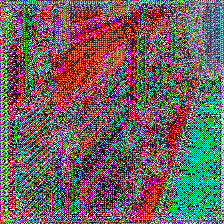
\includegraphics[width=\textwidth]{figures/result/single/depth/1.png}
     \caption{depth}
    \end{subfigure}
    ~
    \begin{subfigure}[b]{0.175\textwidth}
     
\includegraphics[width=\textwidth]{figures/result/single/emissive/1.png}
     \caption{emissive}
    \end{subfigure}
    ~
    \begin{subfigure}[b]{0.175\textwidth}
     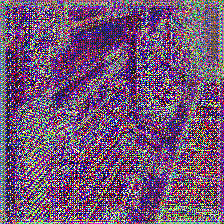
\includegraphics[width=\textwidth]{figures/result/single/metalness/1.png}
     \caption{metalness}
    \end{subfigure}
    \\ \vspace{0.2cm}
    \begin{subfigure}[b]{0.175\textwidth}
     
\includegraphics[width=\textwidth]{figures/result/single/normal/1.png}
     \caption{normal}
    \end{subfigure}
    ~
    \begin{subfigure}[b]{0.175\textwidth}
     
\includegraphics[width=\textwidth]{figures/result/single/position/1.png}
     \caption{position}
    \end{subfigure}
    ~
    \begin{subfigure}[b]{0.175\textwidth}
     
\includegraphics[width=\textwidth]{figures/result/single/roughness/1.png}
     \caption{roughness}
    \end{subfigure}
    \\ \vspace{0.2cm} %2
    \begin{subfigure}[b]{0.175\textwidth}
     
\includegraphics[width=\textwidth]{figures/result/single/albedo/2.png}
     \caption{albedo}\label{subfig:1}
    \end{subfigure}
    ~
    \begin{subfigure}[b]{0.175\textwidth}
     
\includegraphics[width=\textwidth]{figures/result/single/depth/2.png}
     \caption{depth}
    \end{subfigure}
    ~
    \begin{subfigure}[b]{0.175\textwidth}
     
\includegraphics[width=\textwidth]{figures/result/single/emissive/2.png}
     \caption{emissive}
    \end{subfigure}
    ~
    \begin{subfigure}[b]{0.175\textwidth}
     
\includegraphics[width=\textwidth]{figures/result/single/metalness/2.png}
     \caption{metalness}
    \end{subfigure}
    \\ \vspace{0.2cm}
    \begin{subfigure}[b]{0.175\textwidth}
     
\includegraphics[width=\textwidth]{figures/result/single/normal/2.png}
     \caption{normal}
    \end{subfigure}
    ~
    \begin{subfigure}[b]{0.175\textwidth}
     
\includegraphics[width=\textwidth]{figures/result/single/position/2.png}
     \caption{position}
    \end{subfigure}
    ~
    \begin{subfigure}[b]{0.175\textwidth}
     
\includegraphics[width=\textwidth]{figures/result/single/roughness/2.png}
     \caption{roughness}
    \end{subfigure}
    \caption[Generation Result with fixed input on Single input added to EEVEE]{The output generated from RenderGAN with single additional information used in combination with the EEVEE numerical result are reported to Tab.~\ref{tab:render_single_input_table}}
    \label{fig:single_input_generation}
\end{figure}
% double input
% Albedo
\begin{figure}[h!]
    \centering
    % 1
    \begin{subfigure}[b]{0.175\textwidth}
     \includegraphics[width=\textwidth]{figures/result/double/Albedo_Emissive/1.png}
     \caption{Emissive}\label{subfig:1}
    \end{subfigure}
    ~
    \begin{subfigure}[b]{0.175\textwidth}
     \includegraphics[width=\textwidth]{figures/result/double/Albedo_Metalness/1.png}
     \caption{Metalness}
    \end{subfigure}
    ~
    \begin{subfigure}[b]{0.175\textwidth}
     \includegraphics[width=\textwidth]{figures/result/double/Albedo_Normal/1.png}
     \caption{Normal}
    \end{subfigure}
    ~
    \begin{subfigure}[b]{0.175\textwidth}
     \includegraphics[width=\textwidth]{figures/result/double/Albedo_Position/1.png}
     \caption{Position}
    \end{subfigure}
    ~
    \begin{subfigure}[b]{0.175\textwidth}
     \includegraphics[width=\textwidth]{figures/result/double/Albedo_Roughness/1.png}
     \caption{Roughness}
    \end{subfigure}
    \\ \vspace{0.2cm} %2
    \begin{subfigure}[b]{0.175\textwidth}
     
\includegraphics[width=\textwidth]{figures/result/double/Albedo_Emissive/2.png}
     \caption{Emissive}
     \label{subfig:1}
    \end{subfigure}
    ~
    \begin{subfigure}[b]{0.175\textwidth}
     
\includegraphics[width=\textwidth]{figures/result/double/Albedo_Metalness/2.png}
     \caption{Metalness}
    \end{subfigure}
    ~
    \begin{subfigure}[b]{0.175\textwidth}
     
\includegraphics[width=\textwidth]{figures/result/double/Albedo_Normal/2.png}
     \caption{Normal}
    \end{subfigure}
    ~
    \begin{subfigure}[b]{0.175\textwidth}
     
\includegraphics[width=\textwidth]{figures/result/double/Albedo_Position/2.png}
     \caption{Position}
    \end{subfigure}
    ~
    \begin{subfigure}[b]{0.175\textwidth}
     
\includegraphics[width=\textwidth]{figures/result/double/Albedo_Roughness/2.png}
     \caption{Roughness}
    \end{subfigure}
    \caption[Generation Result with fixed input on Albedo]{The output generated from RenderGAN with two additional pieces of information used in combination with the EEVEE. In this picture, the combination first element is fixed on the Albedo information and the second one change. Numerical result are reported to Tab.~\ref{tab:render_double_data}}
    \label{fig:double_input_base_albedo_generation}
\end{figure}

% Depth
\begin{figure}[h!]
    \centering
    % 1
    \begin{subfigure}[b]{0.175\textwidth}
     \includegraphics[width=\textwidth]{figures/result/double/Depth_Albedo/1.png}
     \caption{Albedo}\label{subfig:1}
    \end{subfigure}
    ~
    \begin{subfigure}[b]{0.175\textwidth}
     \includegraphics[width=\textwidth]{figures/result/double/Depth_Metalness/1.png}
     \caption{Metalness}
    \end{subfigure}
    ~
    \begin{subfigure}[b]{0.175\textwidth}
     \includegraphics[width=\textwidth]{figures/result/double/Depth_Normal/1.png}
     \caption{Normal}
    \end{subfigure}
    \\ \vspace{0.2cm}
    \begin{subfigure}[b]{0.175\textwidth}
     \includegraphics[width=\textwidth]{figures/result/double/Depth_Position/1.png}
     \caption{Position}
    \end{subfigure}
    ~
    \begin{subfigure}[b]{0.175\textwidth}
     \includegraphics[width=\textwidth]{figures/result/double/Depth_Roughness/1.png}
     \caption{Roughness}
    \end{subfigure}
    ~
    \begin{subfigure}[b]{0.175\textwidth}
     \includegraphics[width=\textwidth]{figures/result/double/Depth_Emissive/1.png}
     \caption{Emissive}
     \label{subfig:double_input_base_depth_and_emissive1}
    \end{subfigure}
    \\ \vspace{0.2cm} %2
    \begin{subfigure}[b]{0.175\textwidth}
     
\includegraphics[width=\textwidth]{figures/result/double/Depth_Albedo/2.png}
     \caption{Albedo}\label{subfig:1}
    \end{subfigure}
    ~
    \begin{subfigure}[b]{0.175\textwidth}
     \includegraphics[width=\textwidth]{figures/result/double/Depth_Metalness/2.png}
     \caption{Metalness}
    \end{subfigure}
    ~
    \begin{subfigure}[b]{0.175\textwidth}
     \includegraphics[width=\textwidth]{figures/result/double/Depth_Normal/2.png}
     \caption{Normal}
    \end{subfigure}
    \\ \vspace{0.2cm}
    \begin{subfigure}[b]{0.175\textwidth}
     \includegraphics[width=\textwidth]{figures/result/double/Depth_Position/2.png}
     \caption{Position}
    \end{subfigure}
    ~
    \begin{subfigure}[b]{0.175\textwidth}
     \includegraphics[width=\textwidth]{figures/result/double/Depth_Roughness/2.png}
     \caption{Roughness}
    \end{subfigure}
    ~
    \begin{subfigure}[b]{0.175\textwidth}
     \includegraphics[width=\textwidth]{figures/result/double/Depth_Emissive/2.png}
     \caption{Emissive}
     \label{subfig:double_input_base_depth_and_emissive2}
    \end{subfigure}
    \caption[Generation Result with fixed input on Depth]{The output generated from RenderGAN with two additional pieces of information used in combination with the EEVEE. In this picture, the combination first element is fixed on the Depth information and the second one change. Numerical result are reported to Tab.~\ref{tab:render_double_data}}
    \label{fig:double_input_base_depth_generation}
\end{figure}

%Normal
\begin{figure}[h!]
    \centering
    % 1
    \begin{subfigure}[b]{0.175\textwidth}
     \includegraphics[width=\textwidth]{figures/result/double/Normal_Emissive/1.png}
     \caption{Emissive}\label{subfig:1}
    \end{subfigure}
    ~
    \begin{subfigure}[b]{0.175\textwidth}
     \includegraphics[width=\textwidth]{figures/result/double/Normal_Metalness/1.png}
     \caption{Metalness}
    \end{subfigure}
    ~
    \begin{subfigure}[b]{0.175\textwidth}
     \includegraphics[width=\textwidth]{figures/result/double/Normal_Position/1.png}
     \caption{Position}
    \end{subfigure}
    ~
    \begin{subfigure}[b]{0.175\textwidth}
     \includegraphics[width=\textwidth]{figures/result/double/Normal_Roughness/1.png}
     \caption{Roughness}
    \end{subfigure}
    \\ \vspace{0.2cm} %2
    \begin{subfigure}[b]{0.175\textwidth}
     \includegraphics[width=\textwidth]{figures/result/double/Normal_Emissive/1.png}
     \caption{Emissive}\label{subfig:1}
    \end{subfigure}
    ~
    \begin{subfigure}[b]{0.175\textwidth}
     \includegraphics[width=\textwidth]{figures/result/double/Normal_Metalness/1.png}
     \caption{Metalness}
    \end{subfigure}
    ~
    \begin{subfigure}[b]{0.175\textwidth}
     \includegraphics[width=\textwidth]{figures/result/double/Normal_Position/1.png}
     \caption{Position}
    \end{subfigure}
    ~
    \begin{subfigure}[b]{0.175\textwidth}
     \includegraphics[width=\textwidth]{figures/result/double/Normal_Roughness/1.png}
     \caption{Roughness}
    \end{subfigure}
    \caption[Generation Result with fixed input on Normal]{The output generated from RenderGAN with two additional pieces of information used in combination with the EEVEE. In this picture, the combination first element is fixed on the Normal information and the second one change. Numerical result are reported to Tab.~\ref{tab:render_double_data}}
    \label{fig:double_input_base_normal_generation}
\end{figure}

%Emissive
\begin{figure}[h!]
    \centering
    % 1
    \begin{subfigure}[b]{0.175\textwidth}
     \includegraphics[width=\textwidth]{figures/result/double/Emissive_Metalness/1.png}
     \caption{Metalness}\label{subfig:1}
    \end{subfigure}
    ~
    \begin{subfigure}[b]{0.175\textwidth}
     \includegraphics[width=\textwidth]{figures/result/double/Emissive_Position/1.png}
     \caption{Position}
    \end{subfigure}
    ~
    \begin{subfigure}[b]{0.175\textwidth}
     \includegraphics[width=\textwidth]{figures/result/double/Emissive_Roughness/1.png}
     \caption{Roughness}
    \end{subfigure}
    \\ \vspace{0.2cm} %2
    \begin{subfigure}[b]{0.175\textwidth}
     \includegraphics[width=\textwidth]{figures/result/double/Emissive_Metalness/2.png}
     \caption{Metalness}\label{subfig:1}
    \end{subfigure}
    ~
    \begin{subfigure}[b]{0.175\textwidth}
     \includegraphics[width=\textwidth]{figures/result/double/Emissive_Position/2.png}
     \caption{Position}
    \end{subfigure}
    ~
    \begin{subfigure}[b]{0.175\textwidth}
     \includegraphics[width=\textwidth]{figures/result/double/Emissive_Roughness/2.png}
     \caption{Roughness}
    \end{subfigure}
    \caption[Generation Result with fixed input on Emissive]{The output generated from RenderGAN with two additional pieces of information used in combination with the EEVEE. In this picture, the combination first element is fixed on the Emissive information and the second one change. Numerical result are reported to Tab.~\ref{tab:render_double_data}}
    \label{fig:double_input_base_emissive_generation}
\end{figure}

%Metalness
\begin{figure}[h!]
    \centering
    % 1
    \begin{subfigure}[b]{0.175\textwidth}
     \includegraphics[width=\textwidth]{figures/result/double/Metalness_Position/1.png}
     \caption{Position}\label{subfig:1}
    \end{subfigure}
    ~
    \begin{subfigure}[b]{0.175\textwidth}
     \includegraphics[width=\textwidth]{figures/result/double/Metalness_Roughness/1.png}
     \caption{Roughness}
    \end{subfigure}
    ~ 
    %2
    \begin{subfigure}[b]{0.175\textwidth}
     \includegraphics[width=\textwidth]{figures/result/double/Metalness_Position/2.png}
     \caption{Position}\label{subfig:1}
    \end{subfigure}
    ~
    \begin{subfigure}[b]{0.175\textwidth}
     \includegraphics[width=\textwidth]{figures/result/double/Metalness_Roughness/2.png}
     \caption{Roughness}
    \end{subfigure}
    \caption[Generation Result with fixed input on Metalness]{The output generated from RenderGAN with two additional pieces of information used in combination with the EEVEE. In this picture, the combination first element is fixed on the Metalness information and the second one change. Numerical result are reported to Tab.~\ref{tab:render_double_data}}
    \label{fig:double_input_base_metalness_generation}
\end{figure}

% 3
% depth_elbedo
\begin{figure}[h!]
    \centering
    % 1
    \begin{subfigure}[b]{0.175\textwidth}
     \includegraphics[width=\textwidth]{figures/result/triple/depth_albedo_emissive/1.png}
     \caption{Emissive}\label{subfig:1}
    \end{subfigure}
    ~
    \begin{subfigure}[b]{0.175\textwidth}
     \includegraphics[width=\textwidth]{figures/result/triple/depth_albedo_metalness/1.png}
     \caption{Metalness}
    \end{subfigure}
    ~
    \begin{subfigure}[b]{0.175\textwidth}
     \includegraphics[width=\textwidth]{figures/result/triple/depth_albedo_normal/1.png}
     \caption{Normal}
    \end{subfigure}
    \\ \vspace{0.2cm} 
    \begin{subfigure}[b]{0.175\textwidth}
     \includegraphics[width=\textwidth]{figures/result/triple/depth_albedo_position/1.png}
     \caption{Position}\label{subfig:1}
    \end{subfigure}
    ~
    \begin{subfigure}[b]{0.175\textwidth}
     \includegraphics[width=\textwidth]{figures/result/triple/depth_albedo_roughness/1.png}
     \caption{Roughness}
    \end{subfigure}
    %2
    \\ \vspace{0.2cm} %2
    \begin{subfigure}[b]{0.175\textwidth}
     \includegraphics[width=\textwidth]{figures/result/triple/depth_albedo_emissive/2.png}
     \caption{Emissive}\label{subfig:1}
    \end{subfigure}
    ~
    \begin{subfigure}[b]{0.175\textwidth}
     \includegraphics[width=\textwidth]{figures/result/triple/depth_albedo_metalness/2.png}
     \caption{Metalness}
    \end{subfigure}
    ~
    \begin{subfigure}[b]{0.175\textwidth}
     \includegraphics[width=\textwidth]{figures/result/triple/depth_albedo_normal/2.png}
     \caption{Normal}
    \end{subfigure}
    \\ \vspace{0.2cm} %2
    \begin{subfigure}[b]{0.175\textwidth}
     \includegraphics[width=\textwidth]{figures/result/triple/depth_albedo_position/2.png}
     \caption{Position}\label{subfig:1}
    \end{subfigure}
    ~
    \begin{subfigure}[b]{0.175\textwidth}
     \includegraphics[width=\textwidth]{figures/result/triple/depth_albedo_roughness/2.png}
     \caption{Roughness}
    \end{subfigure}
    \caption[Generation Result with fixed input on Depth and Albedo]{The output generated from RenderGAN with three additional pieces of information used in combination with the EEVEE. In this picture the combination first two elements are fixed on the Depth and Albedo information and the second one change. Numerical result are reported to Tab.~\ref{tab:render_triple_data}}
    \label{fig:triple_input_base_depth_albedo}
\end{figure}

%albedo_normal
\begin{figure}[h!]
    \centering
    % 1
    \begin{subfigure}[b]{0.175\textwidth}
     \includegraphics[width=\textwidth]{figures/result/triple/albedo_normal_emissive/1.png}
     \caption{Emissive}\label{subfig:1}
    \end{subfigure}
    ~
    \begin{subfigure}[b]{0.175\textwidth}
     \includegraphics[width=\textwidth]{figures/result/triple/albedo_normal_metalness/1.png}
     \caption{Metalness}
    \end{subfigure}
    ~
    \begin{subfigure}[b]{0.175\textwidth}
     \includegraphics[width=\textwidth]{figures/result/triple/albedo_normal_position/1.png}
     \caption{Position}
    \end{subfigure}
    %2
    \\ \vspace{0.2cm} %2
    \begin{subfigure}[b]{0.175\textwidth}
     \includegraphics[width=\textwidth]{figures/result/triple/albedo_normal_emissive/2.png}
     \caption{Emissive}\label{subfig:1}
    \end{subfigure}
    ~
    \begin{subfigure}[b]{0.175\textwidth}
     \includegraphics[width=\textwidth]{figures/result/triple/albedo_normal_metalness/2.png}
     \caption{Metalness}
    \end{subfigure}
    ~
    \begin{subfigure}[b]{0.175\textwidth}
     \includegraphics[width=\textwidth]{figures/result/triple/albedo_normal_position/2.png}
     \caption{Position}
    \end{subfigure}
    \caption[Generation Result with fixed input on Albedo and Normal]{The output generated from RenderGAN with three additional pieces of information used in combination with the EEVEE. In this picture the combination first two elements are fixed on the Albedo and Normal information and the second one change. Numerical result are reported to Tab.~\ref{tab:render_triple_data}}
    \label{fig:triple_input_base_albedo_normal}
\end{figure}

%normal_emissive
\begin{figure}[h!]
    \centering
    % 1
    \begin{subfigure}[b]{0.175\textwidth}
     \includegraphics[width=\textwidth]{figures/result/triple/normal_emissive_metalness/1.png}
     \caption{Metalness}\label{subfig:1}
    \end{subfigure}
    ~
    \begin{subfigure}[b]{0.175\textwidth}
     \includegraphics[width=\textwidth]{figures/result/triple/normal_emissive_position/1.png}
     \caption{Position}
    \end{subfigure}
    ~
    \begin{subfigure}[b]{0.175\textwidth}
     \includegraphics[width=\textwidth]{figures/result/triple/normal_emissive_roughness/1.png}
     \caption{Roughness}
    \end{subfigure}
    %2
    \\ \vspace{0.2cm} %2
    \begin{subfigure}[b]{0.175\textwidth}
     \includegraphics[width=\textwidth]{figures/result/triple/normal_emissive_metalness/2.png}
     \caption{Metalness}\label{subfig:1}
    \end{subfigure}
    ~
    \begin{subfigure}[b]{0.175\textwidth}
     \includegraphics[width=\textwidth]{figures/result/triple/normal_emissive_position/2.png}
     \caption{Position}
    \end{subfigure}
    ~
    \begin{subfigure}[b]{0.175\textwidth}
     \includegraphics[width=\textwidth]{figures/result/triple/normal_emissive_roughness/3.png}
     \caption{Roughness}
    \end{subfigure}
    \caption[Generation Result with fixed input on Normal and Emissive]{The output generated from RenderGAN with three additional pieces of information used in combination with the EEVEE. In this picture the combination first two elements are fixed on the Normal and Emissive information and the second one change. Numerical result are reported to Tab.~\ref{tab:render_triple_data}}
    \label{fig:triple_input_base_normal_emissive}
\end{figure}

% emissive_metalness
\begin{figure}[h!]
    \centering
    % 1
    \begin{subfigure}[b]{0.175\textwidth}
     \includegraphics[width=\textwidth]{figures/result/triple/emissive_metalness_position/1.png}
     \caption{Position}\label{subfig:1}
    \end{subfigure}
    ~
    \begin{subfigure}[b]{0.175\textwidth}
     \includegraphics[width=\textwidth]{figures/result/triple/emissive_metalness_roughness/1.png}
     \caption{Roughness}
    \end{subfigure} 
    %2
    \\ \vspace{0.2cm} %2
    \begin{subfigure}[b]{0.175\textwidth}
     \includegraphics[width=\textwidth]{figures/result/triple/emissive_metalness_position/2.png}
     \caption{Position}\label{subfig:1}
    \end{subfigure}
    ~
    \begin{subfigure}[b]{0.175\textwidth}
     \includegraphics[width=\textwidth]{figures/result/triple/emissive_metalness_roughness/2.png}
     \caption{Roughness}
    \end{subfigure}
    \caption[Generation Result with fixed input on Emissive and Metalness]{The output generated from RenderGAN with three additional pieces of information used in combination with the EEVEE. In this picture the combination first two elements are fixed on the Emissive and Metalness information and the second one change. Numerical result are reported to Tab.~\ref{tab:render_triple_data}}
    \label{fig:triple_input_base_emissive_metalness}
\end{figure}

%quadruple
% depth_albedo_normal
\begin{figure}[h!]
    \centering
    % 1
    \begin{subfigure}[b]{0.175\textwidth}
     \includegraphics[width=\textwidth]{figures/result/quadruple/depth_albedo_normal_emissive/1.png}
     \caption{Emissive}\label{subfig:1}
    \end{subfigure}
    ~
    \begin{subfigure}[b]{0.175\textwidth}
     \includegraphics[width=\textwidth]{figures/result/quadruple/depth_albedo_normal_metalness/1.png}
     \caption{Metalness}
    \end{subfigure}
    ~
    \begin{subfigure}[b]{0.175\textwidth}
     \includegraphics[width=\textwidth]{figures/result/quadruple/depth_albedo_normal_position/1.png}
     \caption{Position}
    \end{subfigure}
    ~
    \begin{subfigure}[b]{0.175\textwidth}
     \includegraphics[width=\textwidth]{figures/result/quadruple/depth_albedo_normal_roughness/1.png}
     \caption{Roughness}\label{subfig:1}
    \end{subfigure}
    %2
    \\ \vspace{0.2cm}
    \begin{subfigure}[b]{0.175\textwidth}
     \includegraphics[width=\textwidth]{figures/result/quadruple/depth_albedo_normal_emissive/2.png}
     \caption{Emissive}\label{subfig:1}
    \end{subfigure}
    ~
    \begin{subfigure}[b]{0.175\textwidth}
     \includegraphics[width=\textwidth]{figures/result/quadruple/depth_albedo_normal_metalness/2.png}
     \caption{Metalness}
    \end{subfigure}
    ~
    \begin{subfigure}[b]{0.175\textwidth}
     \includegraphics[width=\textwidth]{figures/result/quadruple/depth_albedo_normal_position/2.png}
     \caption{Position}
    \end{subfigure}
    ~
    \begin{subfigure}[b]{0.175\textwidth}
     \includegraphics[width=\textwidth]{figures/result/quadruple/depth_albedo_normal_roughness/2.png}
     \caption{Roughness}\label{subfig:1}
    \end{subfigure}
    
    \caption[Generation Result with fixed input on Depth and Albedo]{The output generated from RenderGAN with four additional pieces of information used in combination with the EEVEE. In this picture the combination first two elements are fixed on the Depth and Albedo and Normal information and the second one change. Numerical result are reported to Tab.~\ref{tab:render_four_data}}
    \label{fig:quadruple_input_base_depth_albedo}
\end{figure}

% albedo_normal_emissive
\begin{figure}[h!]
    \centering
    % 1
    \begin{subfigure}[b]{0.175\textwidth}
     \includegraphics[width=\textwidth]{figures/result/quadruple/albedo_normal_emissive_position/1.png}
     \caption{Position}\label{subfig:1}
    \end{subfigure}
    ~
    \begin{subfigure}[b]{0.175\textwidth}
     \includegraphics[width=\textwidth]{figures/result/quadruple/albedo_normal_emissive_metalness/1.png}
     \caption{Metalness}
    \end{subfigure}
    ~
    \begin{subfigure}[b]{0.175\textwidth}
     \includegraphics[width=\textwidth]{figures/result/quadruple/depth_albedo_normal_roughness/1.png}
     \caption{Roughness}
    \end{subfigure}
    %2
    \\ \vspace{0.2cm}
    \begin{subfigure}[b]{0.175\textwidth}
     \includegraphics[width=\textwidth]{figures/result/quadruple/albedo_normal_emissive_position/2.png}
     \caption{Position}\label{subfig:1}
    \end{subfigure}
    ~
    \begin{subfigure}[b]{0.175\textwidth}
     \includegraphics[width=\textwidth]{figures/result/quadruple/albedo_normal_emissive_metalness/2.png}
     \caption{Metalness}
    \end{subfigure}
    ~
    \begin{subfigure}[b]{0.175\textwidth}
     \includegraphics[width=\textwidth]{figures/result/quadruple/depth_albedo_normal_roughness/2.png}
     \caption{Roughness}
    \end{subfigure}
    
    \caption[Generation Result with fixed input on Albedo and Normal]{The output generated from RenderGAN with four additional information used in combination to the EEVEE. In this picture the combination first two elements is fixed on the Albedo and Normal and Emissive information and the second one change. Numerical result are reported to Tab.~\ref{tab:render_four_data}}
    \label{fig:quadruple_input_base_albedo_normal}
\end{figure}

% normal_emissive_metalness/roughness
\begin{figure}[h!]
    \centering
    % 1
    \begin{subfigure}[b]{0.175\textwidth}
     \includegraphics[width=\textwidth]{figures/result/quadruple/normal_emissive_metalness_position/1.png}
     \caption{Metalness_Position}\label{subfig:1}
    \end{subfigure}
    ~
    \begin{subfigure}[b]{0.175\textwidth}
     \includegraphics[width=\textwidth]{figures/result/quadruple/normal_emissive_metalness_roughness/1.png}
     \caption{Metalness_Roughness}
    \end{subfigure}
    ~
    \begin{subfigure}[b]{0.175\textwidth}
     \includegraphics[width=\textwidth]{figures/result/quadruple/normal_emissive_roughness_position/1.png}
     \caption{Roughness_Position}
     \label{subfig:quadruple_input_base_normal_emissive_roughness_position}
    \end{subfigure}
    \\ \vspace{0.2cm} %2
    \begin{subfigure}[b]{0.175\textwidth}
     \includegraphics[width=\textwidth]{figures/result/quadruple/normal_emissive_metalness_position/2.png}
     \caption{Metalness_Position}
    \end{subfigure}
    ~
    \begin{subfigure}[b]{0.175\textwidth}
     \includegraphics[width=\textwidth]{figures/result/quadruple/normal_emissive_metalness_position/2.png}
     \caption{Metalness_Roughness}
    \end{subfigure}
    ~
    \begin{subfigure}[b]{0.175\textwidth}
     \includegraphics[width=\textwidth]{figures/result/quadruple/normal_emissive_roughness_position/2.png}
     \caption{Roughness_Position}
    \end{subfigure}
    \caption[Generation Result with fixed input on Normal and Emissive]{The output generated from RenderGAN with four additional pieces of information used in combination with the EEVEE. In this picture the combination first two elements are fixed on the Normal and Emissive information and the second one change. Numerical result are reported to Tab.~\ref{tab:render_four_data}}
    \label{fig:quadruple_input_base_normal_emissive}
\end{figure}

\begin{figure}[h!]
    \centering
    % 1
    \begin{subfigure}[b]{0.9\textwidth}
     \includegraphics[width=\textwidth]{figures/result/gt/s9_camera_9_cycles.png}
     \caption{}\label{subfig:1}
    \end{subfigure}
    \\ \vspace{0.2cm}
    \begin{subfigure}[b]{0.9\textwidth}
     \includegraphics[width=\textwidth]{figures/result/gt/s9_camera_80_cycles.png}
     \caption{}
    \end{subfigure}
    \caption[Cycles Render]{The ground truth images for the generated render in Fig.~\ref{fig:RenderGAN_images1}}
    \label{fig:gt_images1}
\end{figure}
\begin{figure}[h!]
    \centering
    \begin{subfigure}[b]{0.9\textwidth}
     \includegraphics[width=\textwidth]{figures/result/gt/s6_camera_60_cycles.png}
     \caption{}
    \end{subfigure}
    \\ \vspace{0.2cm}
    \begin{subfigure}[b]{0.9\textwidth}
     \includegraphics[width=\textwidth]{figures/result/gt/s3_camera_17_cycles.png}
     \caption{}
    \end{subfigure}
    \caption[Cycles Render]{The ground truth images for the generated render in Fig.~\ref{fig:RenderGAN_images2}}
    \label{fig:gt_images2}
\end{figure}
\begin{figure}[h!]
    \centering
    \begin{subfigure}[b]{0.9\textwidth}
     \includegraphics[width=\textwidth]{figures/result/gt/s1_camera_95_cycles.png}
     \caption{}
    \end{subfigure}
    \\ \vspace{0.2cm}
    \begin{subfigure}[b]{0.9\textwidth}
     \includegraphics[width=\textwidth]{figures/result/gt/s1_camera_2_cycles.png}
     \caption{}
    \end{subfigure}
    \caption[Cycles Render]{The ground truth images for the generated render in Fig.~\ref{fig:RenderGAN_images3}}
    \label{fig:gt_images3}
\end{figure}

\begin{figure}[h!]
    \centering
    % 1
    \begin{subfigure}[b]{0.9\textwidth}
     \includegraphics[width=\textwidth]{figures/result/eevee/s9_camera_9_eevee.png}
     \caption{}\label{subfig:1}
    \end{subfigure}
    \\ \vspace{0.2cm}
    \begin{subfigure}[b]{0.9\textwidth}
     \includegraphics[width=\textwidth]{figures/result/eevee/s9_camera_80_eevee.png}
     \caption{}
    \end{subfigure}
\caption[EEVEE Example of input]{The EEVEE input images for the render in Fig.~\ref{fig:RenderGAN_images1}}
    \label{fig:eevee_images1}
\end{figure}
\begin{figure}[h!]
    \centering
    \begin{subfigure}[b]{0.9\textwidth}
     \includegraphics[width=\textwidth]{figures/result/eevee/s6_camera_60_eevee.png}
     \caption{}
    \end{subfigure}
    \\ \vspace{0.2cm}
    \begin{subfigure}[b]{0.9\textwidth}
     \includegraphics[width=\textwidth]{figures/result/eevee/s3_camera_17_eevee.png}
     \caption{}
    \end{subfigure}
\caption[EEVEE Example of input]{The EEVEE input images for the render in Fig.~\ref{fig:RenderGAN_images2}}
    \label{fig:eevee_images2}
\end{figure}
\begin{figure}[h!]
    \centering
    \begin{subfigure}[b]{0.9\textwidth}
     \includegraphics[width=\textwidth]{figures/result/eevee/s1_camera_95_eevee.png}
     \caption{}
    \end{subfigure}
    \\ \vspace{0.2cm}
    \begin{subfigure}[b]{0.9\textwidth}
     \includegraphics[width=\textwidth]{figures/result/eevee/s1_camera_2_eevee.png}
     \caption{}
    \end{subfigure}
    \caption[EEVEE Example of input]{The EEVEE input images for the render in Fig.~\ref{fig:RenderGAN_images3}}
    \label{fig:eevee_images3}
\end{figure}

\begin{figure}[h!]
    \centering
    % 1
    \begin{subfigure}[b]{0.9\textwidth}
     \includegraphics[width=\textwidth]{figures/result/all/s9_camera_9_cycles_RN.png}
     \caption{}\label{subfig:1}
    \end{subfigure}
    \\ \vspace{0.2cm}
    \begin{subfigure}[b]{0.9\textwidth}
     \includegraphics[width=\textwidth]{figures/result/all/s9_camera_80_cycles_RN.png}
     \caption{}
    \end{subfigure}    
    \caption[RenderGAN output]{The RenderGAN output images for the images shown in other pictures but obtained with EEVEE combined with all the other information}
    \label{fig:RenderGAN_images1}
\end{figure}
\begin{figure}[h!]
    \centering
    % 1
    \begin{subfigure}[b]{0.9\textwidth}
     \includegraphics[width=\textwidth]{figures/result/all/s6_camera_60_cycles_RN.png}
     \caption{}\label{subfig:1}
    \end{subfigure}
    \\ \vspace{0.2cm}
    \begin{subfigure}[b]{0.9\textwidth}
     \includegraphics[width=\textwidth]{figures/result/all/s3_camera_17_cycles_RN.png}
     \caption{}
    \end{subfigure}    
    \caption[RenderGAN output]{The RenderGAN output images for the images shown in other pictures but obtained with EEVEE combined with all the other information}
    \label{fig:RenderGAN_images2}
\end{figure}
\begin{figure}[h!]
    \centering
    % 1
    \begin{subfigure}[b]{0.9\textwidth}
     \includegraphics[width=\textwidth]{figures/result/all/s1_camera_95_cycles_RN.png}
     \caption{}\label{subfig:1}
    \end{subfigure}
    \\ \vspace{0.2cm}
    \begin{subfigure}[b]{0.9\textwidth}
     \includegraphics[width=\textwidth]{figures/result/all/s1_camera_2_cycles_RN.png}
     \caption{}
    \end{subfigure}    
    \caption[RenderGAN output]{The RenderGAN output images for the images shown in other pictures but obtained with EEVEE combined with all the other information}
    \label{fig:re
    ndernet_images3}
\end{figure}


To assess the performance and effectiveness of our rendering approach, we employed various image quality evaluation indices. The result presented in Tables~\ref{tab:render_single_input_table},~\ref{tab:render_double_data},~\ref{tab:render_triple_data}, and~\ref{tab:render_four_data} demonstrate that the best outcomes are achieved when using all available input data. Specifically, this confirms that leveraging an encoder composed of convolutional components to extract information from Albedo, Depth, Normal, Emissive, Metalness, and Position yields optimal result. The visualizations in Figures \ref{fig:single_input_generation}, \ref{fig:double_input_base_albedo_generation}, \ref{fig:double_input_base_depth_generation}, \ref{fig:double_input_base_emissive_generation}, \ref{fig:double_input_base_metalness_generation}, \ref{fig:double_input_base_normal_generation}, \ref{fig:triple_input_base_depth_albedo}, \ref{fig:triple_input_base_albedo_normal}, \ref{fig:triple_input_base_emissive_metalness}, \ref{fig:triple_input_base_normal_emissive}, \ref{fig:quadruple_input_base_albedo_normal}, and \ref{fig:quadruple_input_base_depth_albedo}, provide further insights into the impact of different input combinations and the network's performance with 500 epochs of training.

From the visualizations, it is evident that using fewer input data during training (e.g., Albedo and Depth, Albedo and Emissive, etc.) allows the network to learn the structural representation from the input images. However, the reconstruction of colors associated with the structures is compromised. This is evident in the visual examples presented in Figures \ref{fig:double_input_base_albedo_generation} and \ref{fig:double_input_base_depth_generation}. Additionally, analyzing the usefulness of convolutional components for the intermediate data space (Z for Encoder_Decoder architectures), we find that combining EEVEE as input with Albedo, Depth, Emissive, Metalness, Position, and Roughness information allows the network to effectively reconstruct the image structure.

Further analysis reveals that utilizing additional information such as Albedo and Normal, Albedo and Emissive, etc., provides better result in terms of image structure recognition. This is supported by numerical result for SSIM and MSSIM metrics, whereas for Perceptual Loss, Albedo and Normal perform well. Similarly, using Roughness information in combination with Depth yields favorable visual result and is confirmed by the Perceptual Loss value. However, when Emissive is used in combination with other information, the network shows excellent numerical result on average but fails to consistently recognize the structure correctly in visualizations.

Furthermore, the utilization of Normal in combination with other inputs allows the network to recognize the image's structure, but the image reconstruction is not as reliable, except when combined with Position information. On the other hand, Emissive combined with Metalness enables structure recognition and reconstruction, but not entirely. The numerical values confirm these observations. Finally, using four pieces of information as input allows the network to recognize the structure effectively, especially when combining Roughness and Position with Normal and Emissive, as evident in Figure \ref{fig:quadruple_input_base_normal_emissive_roughness_position}.

In evaluating the numerical metrics, it becomes apparent that the values of SSIM and MSSIM are strongly influenced by the recognition of the image structure rather than its content, including brightness, contrast, and shadow gradations. Consequently, the Universal Image Quality Index (UIQI) emerges as the most reliable metric for verifying the correct reconstruction of the rendering. Comparing the generated images (Figures \ref{fig:RenderGAN_images1}, \ref{fig:RenderGAN_images2}, and \ref{fig:RenderGAN_images3}) with the ground truth images (Figures \ref{fig:gt_images1}, \ref{fig:gt_images2}, and \ref{fig:gt_images3}), it is evident that the structural reconstruction is accurate, as supported by the Perceptual Loss and average UIQI values.

Furthermore, the illumination in the generated images, while differing from the expected illumination, allows for correct visualization. This is especially noticeable when the generated images have more lumen than the ground truth images, as the light distribution is better calculated, as demonstrated in Figures \ref{fig:RenderGAN_images1}, \ref{fig:RenderGAN_images2}, and \ref{fig:RenderGAN_images3} compared to Figures \ref{fig:gt_images1}, \ref{fig:gt_images2}, and \ref{fig:gt_images3}. This highlights the significance of the information present in the G_Buffer for improved light distribution in the generated images.

%TODO da modificare
\label{sec:rendering_result}
The training configuration tested on a 40GB A100

The RMSProp optimizer was used as suggested in the Wasserstain GAN framework.
The network was trailed for 500 epochs. Graphs of the loss trend are shown on the x_axis are the steps while on the y_axis are the values achieved. As expected from the discriminator loss it is decreasing and at the end of the training has the value 0.000146. MEntre for the generator the L1 distance reaches a value of 0.009841 with a decreasing monotony. THE perceptual loss has a decreasing trend with minimum value 0.09785.

\begin{figure}[!h]
    \centering
    \begin{subfigure}[b]{0.3\textwidth}
        \includegraphics[width=\textwidth]{result/figures/render/graph/train_discriminator_loss.png}
        \caption{}
        \label{subfig:render_discriminator_loss}
    \end{subfigure}
    ~
    \begin{subfigure}[b]{0.3\textwidth}
        \includegraphics[width=\textwidth]{result/figures/render/graph/train_generator_distance.png}
        \caption{}
        \label{subfig:render_generator_l1}
    \end{subfigure}
    ~
    \begin{subfigure}[b]{0.3\textwidth}
        \includegraphics[width=\textwidth]{result/figures/render/graph/train_perceptual_loss_2.png}
        \caption{}
        \label{subfig:render_generator_perceptual}
    \end{subfigure}
    \caption{Discriminator loss \ref{subfig:render_discriminator_loss} and generator l1 distance in \ref{subfig:render_generator_l1} and perceptual loss in \ref{subfig:render_generator_perceptual}}
    \label{fig:render_loss_training_graph_best}
\end{figure}

\begin{figure}[!h]
    \centering
    \begin{subfigure}[b]{0.3\textwidth}
        \includegraphics[width=\textwidth]{result/figures/render/graph/train_SSIM.png}
        \caption{}
        \label{subfig:render_ssim_metric}
    \end{subfigure}
    ~
    \begin{subfigure}[b]{0.3\textwidth}
        \includegraphics[width=\textwidth]{result/figures/render/graph/train_MSSSIM.png}
        \caption{}
        \label{subfig:render_msssim_metric}
    \end{subfigure}
    \caption{SSIM metric\ref{subfig:render_ssim_metric} and MSSIM in \ref{subfig:render_msssim_metric}}
    \label{fig:render_metrics_training_graph_best}
\end{figure}

As can be seen from the graphs the generator is trained every 3 updates of the discriminator.
The metrics measured in the training phase their trend is shown in the Fig~\ref{fig:render_loss_training_graph_best}

The \textbf{STRUCTURAL SIMILARITY INDEX MEASURE} is used to measure the similarity between 2 images and is defined in \cite{wang2003multiscale} as the \textbf{MULTI_SCALE SSIM} makes use of the SSIM on M scales with scale 1 the input image.

The \textbf{Universal Image Quality Index} is defined in and the equations are given in \cite{universal_image_quality_index}. It is mathematically defined by modeling the image distortion relative to the reference image as a combination of three factors: loss of correlation, luminance distortion, and contrast distortion. If two images f and g are considered as a matrices with M column and N rows containing pixel values $f[i,j]$, $g[i,j]$, respectively $(0 \geqq i > M, 0 \geqq j > N )$, the universal image quality index $Q$ may be calculated as a product of three components:

\begin{equation}
    Q = \frac{\sigma_{fg}}{\sigma_{f}\sigma{g}} * \frac{2\hat{f}\hat{g}}{\hat{f}^2 + \hat{g}^2} * \frac{2\sigma_{f}\sigma_{g}}{\sigma_f^2 + \sigma_g^2}
\end{equation}
where:
\begin{itemize}
    \item first component is the correlation coefficient, which measures the degree of linear correlation between images f and g. It varies in the range [_1,1]. The best value 1 is obtained when f and g are linearly related which means $g[i,j] = af[i,j]+b$ for all possible values of i and j.
    \item second component measure how close the mean luminance is between images
    \item third component measures how similar the contrasts of the images are
\end{itemize}

The trend of these metrics is increasing indicating a progressive improvement in the quality of the images generated by the network. The graphs are in Figure

\subsubsection{Ablation study}

To verify that the result obtained need all input data, an ablation Study was applied on the convolutional layers of the encoder to understand which data are really useful. Data were used individually as well as in combination.

\begin{table}[h!t]
    \centering
    \begin{tabular}{|r||c|c|c|c|c|}
    \toprule
        \multicolumn{1}{|c||}{\textbf{EEVEE}} & \multicolumn{1}{|c|}{\textbf{L1}} & \multicolumn{1}{|c|}{\textbf{\thead{Perceptual\\ Loss}}} & \multicolumn{1}{|c|}{\textbf{SSIM}} & \multicolumn{1}{|c|}{\textbf{MSSIM}} & \multicolumn{1}{|c|}{\textbf{UIQI}} \\
    \midrule
        Albedo & $0,303$ & $1,51$ & $0,695$ & $0,586$ & $0,00087$ \\
        Depth & $0,235$ & $1,62$ & $0,699$ & $0,794$ & $0,003$ \\
        Normal & $0,323$ & $1,68$ & $0,600$ & $0,553$ & $0,00084$ \\
        Emissive & $0,398$ & $1,55$ & $0,719$ & $0,689$ & $0,00011$ \\
        Metalness & $0,368$ & $2,03$ & $0,776$ & $0,708$ & $0,0025$ \\
        Roughness & $0,368$ & $1,88$ & $0,723$ & $0,653$ & $0,00050$ \\
        Position & $0,262$ & $1,45$ & $0,745$ & $0,591$ & $0,00056$ \\
        \textbf{All} & \textbf{$0,009$} & \textbf{$0,09$} & \textbf{$0,912$} & \textbf{$0,982$} & \textbf{$0,898$} \\
    \bottomrule
    \end{tabular}
    \caption{Result of the RenderGAN network with one additional input}
    \label{tab:render_single_input_table}
\end{table}

\begin{table}[h!]
    \centering
    \begin{adjustbox}{width=\textwidth}
    \begin{tabular}{|r||c|c|c|c|c|}
    \toprule
        \multicolumn{1}{|c||}{\textbf{EEVEE}} & \multicolumn{1}{|c|}{\textbf{L1}} & \multicolumn{1}{|c|}{\textbf{\thead{Perceptual\\ Loss}}} & \multicolumn{1}{|c|}{\textbf{SSIM}} & \multicolumn{1}{|c|}{\textbf{MSSIM}} & \multicolumn{1}{|c|}{\textbf{UIQI}} \\
    \midrule
        \textbf{Depth + Normal} & $0,362$ & $1,62$ & $0,651$ & $0,537$ & $0,002$ \\
        \textbf{Depth + Albedo} & $0,244$ & $1,61$ & $0,661$ & $0,663$ & $0,005$ \\
        \textbf{Depth + Emissive} & $0,432$ & $2,29$ & $0,930$ & $0,826$ & $0,001$ \\
        \textbf{Depth + Metalness} & $0,501$ & $2,20$ & $0,773$ & $0,598$ & $0,0005$ \\
        \textbf{Depth + Roughness} & $0,408$ & $1,51$ & $0,735$ & $0,598$ & $0,0005$ \\
        \textbf{Depth + Position} & $0,392$ & $2,10$ & $0,756$ & $0,671$ & $0,001$ \\
        \textbf{Albedo + Normal} & $0,305$ & $1,57$ & $0,633$ & $0,549$ & $0,001$ \\
        \textbf{Albedo + Emissive} & $0,449$ & $2,53$ & $0,913$ & $0,836$ & $0,0005$ \\
        \textbf{Albedo + Metalness} & $0,409$ & $2,09$ & $0,687$ & $0,637$ & $0,001$ \\
        \textbf{Albedo + Roughness} & $0,398$ & $2,11$ & $0,601$ & $0,605$ & $0,005$ \\
        \textbf{Albedo + Position} & $0,414$ & $2,12$ & $0,664$ & $0,607$ & $0,0001$ \\
        \textbf{Normal + Emissive} & $0,406$ & $1,98$ & $0,883$ & $0,688$ & $0,0003$ \\
        \textbf{Normal + Metalness} & $0,494$ & $2,39$ & $0,661$ & $0,559$ & $0,0003$ \\
        \textbf{Normal + Roughness} & $0,612$ & $2,10$ & $0,624$ & $0,515$ & $0,0004$ \\
        \textbf{Normal + Position} & $0,454$ & $2,15$ & $0,622$ & $0,597$ & $0,0009$ \\
        \textbf{Emissive + Metalness} & $0,349$ & $2,25$ & $0,895$ & $0,775$ & $0,003$ \\
        \textbf{Emissive + Roughness} & $0,283$ & $2,09$ & $0,900$ & $0,837$ & $0,002$ \\
        \textbf{Emissive + Position} & $0,445$ & $1,90$ & $0,922$ & $0,823$ & $0,0008$ \\
        \textbf{Metalness + Roughness} & $0,590$ & $2,29$ & $0,275$ & $0,901$ & $0,0001$ \\
        \textbf{Metalness + Psotion} & $0,443$ & $2,31$ & $0,716$ & $0,649$ & $0,0009$ \\
    \bottomrule
    \end{tabular}
    \end{adjustbox}
    
    \caption{RenderGAN result on double input data}
    \label{tab:render_double_data}
\end{table}

\begin{table}[h!]
    \centering
    \begin{adjustbox}{width=\textwidth}
    \begin{tabular}{|r||c|c|c|c|c|}
    \toprule
        \multicolumn{1}{|c||}{\textbf{EEVEE}} & \multicolumn{1}{|c|}{\textbf{L1}} & \multicolumn{1}{|c|}{\textbf{\thead{Perceptual\\ Loss}}} & \multicolumn{1}{|c|}{\textbf{SSIM}} & \multicolumn{1}{|c|}{\textbf{MSSIM}} & \multicolumn{1}{|c|}{\textbf{UIQI}} \\
    \midrule
        \textbf{Depth + Albedo + Normal} & $0,285$ & $1,71$ & $0,606$ & $0,640$ & $0,004$ \\
        \textbf{Depth + Albedo + Emissive} & $0,220$ & $0,98$ & $0,870$ & $0,736$ & $0,002$ \\
        \textbf{Depth + Albedo + Metalness} & $0,227$ & $1,56$ & $0,715$ & $0,708$ & $0,006$ \\
        \textbf{Depth + Albedo + Roughness} & $0,300$ & $1,23$ & $0,667$ & $0,575$ & $0,001$ \\
        \textbf{Depth + Albedo + Position} & $0,305$ & $1,64$ & $0,692$ & $0,643$ & $0,002$ \\
        \textbf{Albedo + Normal + Metalness} & $0,229$ & $1,36$ & $0,686$ & $0,679$ & $0,007$ \\
        \textbf{Albedo + Normal + Emissive} & $0,289$ & $1,53$ & $0,852$ & $0,675$ & $0,001$ \\
        \textbf{Albedo + Normal + Roughness} & $0,167$ & $1,27$ & $0,622$ & $0,677$ & $0,011$ \\
        \textbf{Albedo + Normal + Position} & $0,239$ & $1,77$ & $0,528$ & $0,612$ & $0,006$ \\
        \textbf{Normal + Emissive + Metalness} & $0,318$ & $1,83$ & $0,856$ & $0,767$ & $0,004$ \\
        \textbf{Normal + Emissive + Roughness} & $0,286$ & $1,46$ & $0,869$ & $0,701$ & $0,002$ \\
        \textbf{Normal + Emissive + Position} & $0,250$ & $1,55$ & $0,813$ & $0,678$ & $0,002$ \\
        \textbf{Emissive + Metalness + Roughness} & $0,244$ & $1,07$ & $0,864$ & $0,681$ & $0,0001$ \\
        \textbf{Emissive + Metalness + Position} & $0,229$ & $1,32$ & $0,862$ & $0,732$ & $0,003$ \\
    \bottomrule
    \end{tabular}
    \end{adjustbox}
    \caption{RenderGAN result on triple input data}
    \label{tab:render_triple_data}
\end{table}

\begin{table}[h!]
    \centering
    \begin{adjustbox}{width=\textwidth}
    \begin{tabular}{|r||c|c|c|c|c|}
    \toprule
        \multicolumn{1}{|c||}{\textbf{EEVEE}} & \multicolumn{1}{|c|}{\textbf{L1}} & \multicolumn{1}{|c|}{\textbf{\thead{Perceptual\\ Loss}}} & \multicolumn{1}{|c|}{\textbf{SSIM}} & \multicolumn{1}{|c|}{\textbf{MSSIM}} & \multicolumn{1}{|c|}{\textbf{UIQI}} \\
    \midrule
        \textbf{Depth + Albedo + Normal + Emissive} & $0,224$ & $0,94$ & $0,638$ & $0,508$ & $0,0005$ \\
        \textbf{Depth + Albedo + Normal + Metalness} & $0,290$ & $0,94$ & $0,874$ & $0,644$ & $0,001$ \\
        \textbf{Depth + Albedo + Normal + Roughness} & $0,241$ & $1,46$ & $0,534$ & $0,549$ & $0,002$ \\
        \textbf{Depth + Albedo + Normal + Position} & $0,305$ & $1,52$ & $0,678$ & $0,641$ & $0,003$ \\
        \textbf{Albedo + Normal + Emissive + Metalness} & $0,247$ & $1,80$ & $0,783$ & $0,688$ & $0,002$ \\
        \textbf{Albedo + Normal + Emissive + Roughness} & $0,304$ & $1,87$ & $0,864$ & $0,780$ & $0,004$ \\
        \textbf{Albedo + Normal + Emissive + Position} & $0,390$ & $1,95$ & $0,838$ & $0,712$ & $0,002$ \\
        \textbf{Normal + Emissive + Metalness + Roughness} & $0,249$ & $1,81$ & $0,816$ & $0,772$ & $0,006$ \\
        \textbf{Normal + Emissive + Metalness + Position} & $0,278$ & $1,41$ & $0,899$ & $0,805$ & $0,004$ \\
        \textbf{Emissive + Metalness + Roughness + Position} & $0,257$ & $1,14$ & $0,826$ & $0,691$ & $0,001$ \\
    \bottomrule
    \end{tabular}
    \end{adjustbox}
    \caption{RenderGAN result on four input data}
    \label{tab:render_four_data}
\end{table}


From the images it is possible to verify that.

% \begin{figure}
%     \centering
%     \begin{subfigure}[b]{0.33\textwidth}
%      \includegraphics[width=\textwidth]{result/figures/render/gt/1.png}
%     \end{subfigure}
%     \begin{subfigure}[b]{0.33\textwidth}
%      \includegraphics[width=\textwidth]{result/figures/render/gt/2.png}
%     \end{subfigure}
%     \begin{subfigure}[b]{0.33\textwidth}
%      \includegraphics[width=\textwidth]{result/figures/render/all/2.jpg}
%     \end{subfigure}
%     \begin{subfigure}[b]{0.33\textwidth}
%      \includegraphics[width=\textwidth]{result/figures/render/all/1.jpg}
%     \end{subfigure}
%     \begin{subfigure}[b]{0.33\textwidth}
%      \includegraphics[width=\textwidth]{result/figures/render/only_eevee/fake_8.png}
%     \end{subfigure}
%     \begin{subfigure}[b]{0.33\textwidth}
%      \includegraphics[width=\textwidth]{result/figures/render/only_eevee/fake_11.png}
%     \end{subfigure}
%     \begin{subfigure}[b]{0.33\textwidth}
%      \includegraphics[width=\textwidth]{result/figures/render/singledata/albedo/1.png}
%     \end{subfigure}
%     \begin{subfigure}[b]{0.33\textwidth}
%      \includegraphics[width=\textwidth]{result/figures/render/singledata/albedo/2.png}
%     \end{subfigure}
%     \begin{subfigure}[b]{0.33\textwidth}
%      \includegraphics[width=\textwidth]{result/figures/render/singledata/depth/1.png}
%     \end{subfigure}
%     \begin{subfigure}[b]{0.33\textwidth}
%      \includegraphics[width=\textwidth]{result/figures/render/singledata/depth/2.png}
%     \end{subfigure}
%     \caption{Caption}
%     \label{fig:my_label}
% \end{figure}

\begin{figure}[h!]
    \centering
    % 1
    \begin{subfigure}[b]{0.175\textwidth}
     \includegraphics[width=\textwidth]{figures/result/single/albedo/1.png}
     \caption{albedo}\label{subfig:1}
    \end{subfigure}
    ~
    \begin{subfigure}[b]{0.175\textwidth}
     \includegraphics[width=\textwidth]{figures/result/single/depth/1.png}
     \caption{depth}
    \end{subfigure}
    ~
    \begin{subfigure}[b]{0.175\textwidth}
     \includegraphics[width=\textwidth]{figures/result/single/emissive/1.png}
     \caption{emissive}
    \end{subfigure}
    ~
    \begin{subfigure}[b]{0.175\textwidth}
     \includegraphics[width=\textwidth]{figures/result/single/metalness/1.png}
     \caption{metalness}
    \end{subfigure}
    \\ \vspace{0.2cm}
    \begin{subfigure}[b]{0.175\textwidth}
     \includegraphics[width=\textwidth]{figures/result/single/normal/1.png}
     \caption{normal}
    \end{subfigure}
    ~
    \begin{subfigure}[b]{0.175\textwidth}
     \includegraphics[width=\textwidth]{figures/result/single/position/1.png}
     \caption{position}
    \end{subfigure}
    ~
    \begin{subfigure}[b]{0.175\textwidth}
     \includegraphics[width=\textwidth]{figures/result/single/roughness/1.png}
     \caption{roughness}
    \end{subfigure}
    \\ \vspace{0.2cm} %2
    \begin{subfigure}[b]{0.175\textwidth}
     \includegraphics[width=\textwidth]{figures/result/single/albedo/2.png}
     \caption{albedo}\label{subfig:1}
    \end{subfigure}
    ~
    \begin{subfigure}[b]{0.175\textwidth}
     \includegraphics[width=\textwidth]{figures/result/single/depth/2.png}
     \caption{depth}
    \end{subfigure}
    ~
    \begin{subfigure}[b]{0.175\textwidth}
     \includegraphics[width=\textwidth]{figures/result/single/emissive/2.png}
     \caption{emissive}
    \end{subfigure}
    ~
    \begin{subfigure}[b]{0.175\textwidth}
     \includegraphics[width=\textwidth]{figures/result/single/metalness/2.png}
     \caption{metalness}
    \end{subfigure}
    \\ \vspace{0.2cm}
    \begin{subfigure}[b]{0.175\textwidth}
     \includegraphics[width=\textwidth]{figures/result/single/normal/2.png}
     \caption{normal}
    \end{subfigure}
    ~
    \begin{subfigure}[b]{0.175\textwidth}
     \includegraphics[width=\textwidth]{figures/result/single/position/2.png}
     \caption{position}
    \end{subfigure}
    ~
    \begin{subfigure}[b]{0.175\textwidth}
     \includegraphics[width=\textwidth]{figures/result/single/roughness/2.png}
     \caption{roughness}
    \end{subfigure}
    \caption{The output generated from RenderNet with single additional information used in combination to the EEVEE numerical result are reported to Tab.~\ref{tab:render_single_input_table}}
    \label{fig:single_input_generation}
\end{figure}
% double input
% Albedo
\begin{figure}[h!]
    \centering
    % 1
    \begin{subfigure}[b]{0.175\textwidth}
     \includegraphics[width=\textwidth]{figures/result/double/Albedo_Emissive/1.png}
     \caption{Emissive}\label{subfig:1}
    \end{subfigure}
    ~
    \begin{subfigure}[b]{0.175\textwidth}
     \includegraphics[width=\textwidth]{figures/result/double/Albedo_Metalness/1.png}
     \caption{Metalness}
    \end{subfigure}
    ~
    \begin{subfigure}[b]{0.175\textwidth}
     \includegraphics[width=\textwidth]{figures/result/double/Albedo_Normal/1.png}
     \caption{Normal}
    \end{subfigure}
    ~
    \begin{subfigure}[b]{0.175\textwidth}
     \includegraphics[width=\textwidth]{figures/result/double/Albedo_Position/1.png}
     \caption{Position}
    \end{subfigure}
    ~
    \begin{subfigure}[b]{0.175\textwidth}
     \includegraphics[width=\textwidth]{figures/result/double/Albedo_Roughness/1.png}
     \caption{Roughness}
    \end{subfigure}
    \\ \vspace{0.2cm} %2
    \begin{subfigure}[b]{0.175\textwidth}
     \includegraphics[width=\textwidth]{figures/result/double/Albedo_Emissive/2.png}
     \caption{Emissive}
     \label{subfig:1}
    \end{subfigure}
    ~
    \begin{subfigure}[b]{0.175\textwidth}
     \includegraphics[width=\textwidth]{figures/result/double/Albedo_Metalness/2.png}
     \caption{Metalness}
    \end{subfigure}
    ~
    \begin{subfigure}[b]{0.175\textwidth}
     \includegraphics[width=\textwidth]{figures/result/double/Albedo_Normal/2.png}
     \caption{Normal}
    \end{subfigure}
    ~
    \begin{subfigure}[b]{0.175\textwidth}
     \includegraphics[width=\textwidth]{figures/result/double/Albedo_Position/2.png}
     \caption{Position}
    \end{subfigure}
    ~
    \begin{subfigure}[b]{0.175\textwidth}
     \includegraphics[width=\textwidth]{figures/result/double/Albedo_Roughness/2.png}
     \caption{Roughness}
    \end{subfigure}
    \caption{The output generated from RenderNet with two additional information used in combination to the EEVEE. In this picture the combination first element is fixed on the Albedo information and the second one change. Numerical result are reported to Tab.~\ref{tab:render_double_data}}
    \label{fig:double_input_base_albedo_generation}
\end{figure}

% Depth
\begin{figure}[h!]
    \centering
    % 1
    \begin{subfigure}[b]{0.175\textwidth}
     \includegraphics[width=\textwidth]{figures/result/double/Depth_Albedo/1.png}
     \caption{Albedo}\label{subfig:1}
    \end{subfigure}
    ~
    \begin{subfigure}[b]{0.175\textwidth}
     \includegraphics[width=\textwidth]{figures/result/double/Depth_Metalness/1.png}
     \caption{Metalness}
    \end{subfigure}
    ~
    \begin{subfigure}[b]{0.175\textwidth}
     \includegraphics[width=\textwidth]{figures/result/double/Depth_Normal/1.png}
     \caption{Normal}
    \end{subfigure}
    \\ \vspace{0.2cm}
    \begin{subfigure}[b]{0.175\textwidth}
     \includegraphics[width=\textwidth]{figures/result/double/Depth_Position/1.png}
     \caption{Position}
    \end{subfigure}
    ~
    \begin{subfigure}[b]{0.175\textwidth}
     \includegraphics[width=\textwidth]{figures/result/double/Depth_Roughness/1.png}
     \caption{Roughness}
    \end{subfigure}
    ~
    \begin{subfigure}[b]{0.175\textwidth}
     \includegraphics[width=\textwidth]{figures/result/double/Depth_Emissive/1.png}
     \caption{Emissive}
     \label{subfig:double_input_base_depth_and_emissive1}
    \end{subfigure}
    \\ \vspace{0.2cm} %2
    \begin{subfigure}[b]{0.175\textwidth}
     \includegraphics[width=\textwidth]{figures/result/double/Depth_Albedo/2.png}
     \caption{Albedo}\label{subfig:1}
    \end{subfigure}
    ~
    \begin{subfigure}[b]{0.175\textwidth}
     \includegraphics[width=\textwidth]{figures/result/double/Depth_Metalness/2.png}
     \caption{Metalness}
    \end{subfigure}
    ~
    \begin{subfigure}[b]{0.175\textwidth}
     \includegraphics[width=\textwidth]{figures/result/double/Depth_Normal/2.png}
     \caption{Normal}
    \end{subfigure}
    \\ \vspace{0.2cm}
    \begin{subfigure}[b]{0.175\textwidth}
     \includegraphics[width=\textwidth]{figures/result/double/Depth_Position/2.png}
     \caption{Position}
    \end{subfigure}
    ~
    \begin{subfigure}[b]{0.175\textwidth}
     \includegraphics[width=\textwidth]{figures/result/double/Depth_Roughness/2.png}
     \caption{Roughness}
    \end{subfigure}
    ~
    \begin{subfigure}[b]{0.175\textwidth}
     \includegraphics[width=\textwidth]{figures/result/double/Depth_Emissive/2.png}
     \caption{Emissive}
     \label{subfig:double_input_base_depth_and_emissive2}
    \end{subfigure}
    \caption{The output generated from RenderNet with two additional information used in combination to the EEVEE. In this picture the combination first element is fixed on the Depth information and the second one change. Numerical result are reported to Tab.~\ref{tab:render_double_data}}
    \label{fig:double_input_base_depth_generation}
\end{figure}

%Normal
\begin{figure}[h!]
    \centering
    % 1
    \begin{subfigure}[b]{0.175\textwidth}
     \includegraphics[width=\textwidth]{figures/result/double/Normal_Emissive/1.png}
     \caption{Emissive}\label{subfig:1}
    \end{subfigure}
    ~
    \begin{subfigure}[b]{0.175\textwidth}
     \includegraphics[width=\textwidth]{figures/result/double/Normal_Metalness/1.png}
     \caption{Metalness}
    \end{subfigure}
    ~
    \begin{subfigure}[b]{0.175\textwidth}
     \includegraphics[width=\textwidth]{figures/result/double/Normal_Position/1.png}
     \caption{Position}
    \end{subfigure}
    ~
    \begin{subfigure}[b]{0.175\textwidth}
     \includegraphics[width=\textwidth]{figures/result/double/Normal_Roughness/1.png}
     \caption{Roughness}
    \end{subfigure}
    \\ \vspace{0.2cm} %2
    \begin{subfigure}[b]{0.175\textwidth}
     \includegraphics[width=\textwidth]{figures/result/double/Normal_Emissive/1.png}
     \caption{Emissive}\label{subfig:1}
    \end{subfigure}
    ~
    \begin{subfigure}[b]{0.175\textwidth}
     \includegraphics[width=\textwidth]{figures/result/double/Normal_Metalness/1.png}
     \caption{Metalness}
    \end{subfigure}
    ~
    \begin{subfigure}[b]{0.175\textwidth}
     \includegraphics[width=\textwidth]{figures/result/double/Normal_Position/1.png}
     \caption{Position}
    \end{subfigure}
    ~
    \begin{subfigure}[b]{0.175\textwidth}
     \includegraphics[width=\textwidth]{figures/result/double/Normal_Roughness/1.png}
     \caption{Roughness}
    \end{subfigure}
    \caption{The output generated from RenderNet with two additional information used in combination to the EEVEE. In this picture the combination first element is fixed on the Normal information and the second one change. Numerical result are reported to Tab.~\ref{tab:render_double_data}}
    \label{fig:double_input_base_normal_generation}
\end{figure}

%Emissive
\begin{figure}[h!]
    \centering
    % 1
    \begin{subfigure}[b]{0.175\textwidth}
     \includegraphics[width=\textwidth]{figures/result/double/Emissive_Metalness/1.png}
     \caption{Metalness}\label{subfig:1}
    \end{subfigure}
    ~
    \begin{subfigure}[b]{0.175\textwidth}
     \includegraphics[width=\textwidth]{figures/result/double/Emissive_Position/1.png}
     \caption{Position}
    \end{subfigure}
    ~
    \begin{subfigure}[b]{0.175\textwidth}
     \includegraphics[width=\textwidth]{figures/result/double/Emissive_Roughness/1.png}
     \caption{Roughness}
    \end{subfigure}
    \\ \vspace{0.2cm} %2
    \begin{subfigure}[b]{0.175\textwidth}
     \includegraphics[width=\textwidth]{figures/result/double/Emissive_Metalness/2.png}
     \caption{Metalness}\label{subfig:1}
    \end{subfigure}
    ~
    \begin{subfigure}[b]{0.175\textwidth}
     \includegraphics[width=\textwidth]{figures/result/double/Emissive_Position/2.png}
     \caption{Position}
    \end{subfigure}
    ~
    \begin{subfigure}[b]{0.175\textwidth}
     \includegraphics[width=\textwidth]{figures/result/double/Emissive_Roughness/2.png}
     \caption{Roughness}
    \end{subfigure}
    \caption{The output generated from RenderNet with two additional information used in combination to the EEVEE. In this picture the combination first element is fixed on the Emissive information and the second one change. Numerical result are reported to Tab.~\ref{tab:render_double_data}}
    \label{fig:double_input_base_emissive_generation}
\end{figure}

%Metalness
\begin{figure}[h!]
    \centering
    % 1
    \begin{subfigure}[b]{0.175\textwidth}
     \includegraphics[width=\textwidth]{figures/result/double/Metalness_Position/1.png}
     \caption{Position}\label{subfig:1}
    \end{subfigure}
    ~
    \begin{subfigure}[b]{0.175\textwidth}
     \includegraphics[width=\textwidth]{figures/result/double/Metalness_Roughness/1.png}
     \caption{Roughness}
    \end{subfigure}
    ~ 
    %2
    \begin{subfigure}[b]{0.175\textwidth}
     \includegraphics[width=\textwidth]{figures/result/double/Metalness_Position/2.png}
     \caption{Position}\label{subfig:1}
    \end{subfigure}
    ~
    \begin{subfigure}[b]{0.175\textwidth}
     \includegraphics[width=\textwidth]{figures/result/double/Metalness_Roughness/2.png}
     \caption{Roughness}
    \end{subfigure}
    \caption{The output generated from RenderNet with two additional information used in combination to the EEVEE. In this picture the combination first element is fixed on the Metalness information and the second one change. Numerical result are reported to Tab.~\ref{tab:render_double_data}}
    \label{fig:double_input_base_metalness_generation}
\end{figure}

% 3
% depth_elbedo
\begin{figure}[h!]
    \centering
    % 1
    \begin{subfigure}[b]{0.175\textwidth}
     \includegraphics[width=\textwidth]{figures/result/triple/depth_albedo_emissive/1.png}
     \caption{Emissive}\label{subfig:1}
    \end{subfigure}
    ~
    \begin{subfigure}[b]{0.175\textwidth}
     \includegraphics[width=\textwidth]{figures/result/triple/depth_albedo_metalness/1.png}
     \caption{Metalness}
    \end{subfigure}
    ~
    \begin{subfigure}[b]{0.175\textwidth}
     \includegraphics[width=\textwidth]{figures/result/triple/depth_albedo_normal/1.png}
     \caption{Normal}
    \end{subfigure}
    \\ \vspace{0.2cm} 
    \begin{subfigure}[b]{0.175\textwidth}
     \includegraphics[width=\textwidth]{figures/result/triple/depth_albedo_position/1.png}
     \caption{Position}\label{subfig:1}
    \end{subfigure}
    ~
    \begin{subfigure}[b]{0.175\textwidth}
     \includegraphics[width=\textwidth]{figures/result/triple/depth_albedo_roughness/1.png}
     \caption{Roughness}
    \end{subfigure}
    %2
    \\ \vspace{0.2cm} %2
    \begin{subfigure}[b]{0.175\textwidth}
     \includegraphics[width=\textwidth]{figures/result/triple/depth_albedo_emissive/2.png}
     \caption{Emissive}\label{subfig:1}
    \end{subfigure}
    ~
    \begin{subfigure}[b]{0.175\textwidth}
     \includegraphics[width=\textwidth]{figures/result/triple/depth_albedo_metalness/2.png}
     \caption{Metalness}
    \end{subfigure}
    ~
    \begin{subfigure}[b]{0.175\textwidth}
     \includegraphics[width=\textwidth]{figures/result/triple/depth_albedo_normal/2.png}
     \caption{Normal}
    \end{subfigure}
    \\ \vspace{0.2cm} %2
    \begin{subfigure}[b]{0.175\textwidth}
     \includegraphics[width=\textwidth]{figures/result/triple/depth_albedo_position/2.png}
     \caption{Position}\label{subfig:1}
    \end{subfigure}
    ~
    \begin{subfigure}[b]{0.175\textwidth}
     \includegraphics[width=\textwidth]{figures/result/triple/depth_albedo_roughness/2.png}
     \caption{Roughness}
    \end{subfigure}
    \caption{The output generated from RenderNet with three additional information used in combination to the EEVEE. In this picture the combination first two elements is fixed on the Depth and Albedo information and the second one change. Numerical result are reported to Tab.~\ref{tab:render_triple_data}}
    \label{fig:triple_input_base_depth_albedo}
\end{figure}

%albedo_normal
\begin{figure}[h!]
    \centering
    % 1
    \begin{subfigure}[b]{0.175\textwidth}
     \includegraphics[width=\textwidth]{figures/result/triple/albedo_normal_emissive/1.png}
     \caption{Emissive}\label{subfig:1}
    \end{subfigure}
    ~
    \begin{subfigure}[b]{0.175\textwidth}
     \includegraphics[width=\textwidth]{figures/result/triple/albedo_normal_metalness/1.png}
     \caption{Metalness}
    \end{subfigure}
    ~
    \begin{subfigure}[b]{0.175\textwidth}
     \includegraphics[width=\textwidth]{figures/result/triple/albedo_normal_position/1.png}
     \caption{Position}
    \end{subfigure}
    %2
    \\ \vspace{0.2cm} %2
    \begin{subfigure}[b]{0.175\textwidth}
     \includegraphics[width=\textwidth]{figures/result/triple/albedo_normal_emissive/2.png}
     \caption{Emissive}\label{subfig:1}
    \end{subfigure}
    ~
    \begin{subfigure}[b]{0.175\textwidth}
     \includegraphics[width=\textwidth]{figures/result/triple/albedo_normal_metalness/2.png}
     \caption{Metalness}
    \end{subfigure}
    ~
    \begin{subfigure}[b]{0.175\textwidth}
     \includegraphics[width=\textwidth]{figures/result/triple/albedo_normal_position/2.png}
     \caption{Position}
    \end{subfigure}
    \caption{The output generated from RenderNet with three additional information used in combination to the EEVEE. In this picture the combination first two elements is fixed on the Albedo and Normal information and the second one change. Numerical result are reported to Tab.~\ref{tab:render_triple_data}}
    \label{fig:triple_input_base_albedo_normal}
\end{figure}

%normal_emissive
\begin{figure}[h!]
    \centering
    % 1
    \begin{subfigure}[b]{0.175\textwidth}
     \includegraphics[width=\textwidth]{figures/result/triple/normal_emissive_metalness/1.png}
     \caption{Metalness}\label{subfig:1}
    \end{subfigure}
    ~
    \begin{subfigure}[b]{0.175\textwidth}
     \includegraphics[width=\textwidth]{figures/result/triple/normal_emissive_position/1.png}
     \caption{Position}
    \end{subfigure}
    ~
    \begin{subfigure}[b]{0.175\textwidth}
     \includegraphics[width=\textwidth]{figures/result/triple/normal_emissive_roughness/1.png}
     \caption{Roughness}
    \end{subfigure}
    %2
    \\ \vspace{0.2cm} %2
    \begin{subfigure}[b]{0.175\textwidth}
     \includegraphics[width=\textwidth]{figures/result/triple/normal_emissive_metalness/2.png}
     \caption{Metalness}\label{subfig:1}
    \end{subfigure}
    ~
    \begin{subfigure}[b]{0.175\textwidth}
     \includegraphics[width=\textwidth]{figures/result/triple/normal_emissive_position/2.png}
     \caption{Position}
    \end{subfigure}
    ~
    \begin{subfigure}[b]{0.175\textwidth}
     \includegraphics[width=\textwidth]{figures/result/triple/normal_emissive_roughness/3.png}
     \caption{Roughness}
    \end{subfigure}
    \caption{The output generated from RenderNet with three additional information used in combination to the EEVEE. In this picture the combination first two elements is fixed on the Normal and Emissive information and the second one change. Numerical result are reported to Tab.~\ref{tab:render_triple_data}}
    \label{fig:triple_input_base_normal_emissive}
\end{figure}

% emissive_metalness
\begin{figure}[h!]
    \centering
    % 1
    \begin{subfigure}[b]{0.175\textwidth}
     \includegraphics[width=\textwidth]{figures/result/triple/emissive_metalness_position/1.png}
     \caption{Position}\label{subfig:1}
    \end{subfigure}
    ~
    \begin{subfigure}[b]{0.175\textwidth}
     \includegraphics[width=\textwidth]{figures/result/triple/emissive_metalness_roughness/1.png}
     \caption{Roughness}
    \end{subfigure} 
    %2
    \\ \vspace{0.2cm} %2
    \begin{subfigure}[b]{0.175\textwidth}
     \includegraphics[width=\textwidth]{figures/result/triple/emissive_metalness_position/2.png}
     \caption{Position}\label{subfig:1}
    \end{subfigure}
    ~
    \begin{subfigure}[b]{0.175\textwidth}
     \includegraphics[width=\textwidth]{figures/result/triple/emissive_metalness_roughness/2.png}
     \caption{Roughness}
    \end{subfigure}
    \caption{The output generated from RenderNet with three additional information used in combination to the EEVEE. In this picture the combination first two elements is fixed on the Emissive and Metalness information and the second one change. Numerical result are reported to Tab.~\ref{tab:render_triple_data}}
    \label{fig:triple_input_base_emissive_metalness}
\end{figure}

%quadruple
% depth_albedo_normal
\begin{figure}[h!]
    \centering
    % 1
    \begin{subfigure}[b]{0.175\textwidth}
     \includegraphics[width=\textwidth]{figures/result/quadruple/depth_albedo_normal_emissive/1.png}
     \caption{Emissive}\label{subfig:1}
    \end{subfigure}
    ~
    \begin{subfigure}[b]{0.175\textwidth}
     \includegraphics[width=\textwidth]{figures/result/quadruple/depth_albedo_normal_metalness/1.png}
     \caption{Metalness}
    \end{subfigure}
    ~
    \begin{subfigure}[b]{0.175\textwidth}
     \includegraphics[width=\textwidth]{figures/result/quadruple/depth_albedo_normal_position/1.png}
     \caption{Position}
    \end{subfigure}
    ~
    \begin{subfigure}[b]{0.175\textwidth}
     \includegraphics[width=\textwidth]{figures/result/quadruple/depth_albedo_normal_roughness/1.png}
     \caption{Roughness}\label{subfig:1}
    \end{subfigure}
    %2
    \\ \vspace{0.2cm}
    \begin{subfigure}[b]{0.175\textwidth}
     \includegraphics[width=\textwidth]{figures/result/quadruple/depth_albedo_normal_emissive/2.png}
     \caption{Emissive}\label{subfig:1}
    \end{subfigure}
    ~
    \begin{subfigure}[b]{0.175\textwidth}
     \includegraphics[width=\textwidth]{figures/result/quadruple/depth_albedo_normal_metalness/2.png}
     \caption{Metalness}
    \end{subfigure}
    ~
    \begin{subfigure}[b]{0.175\textwidth}
     \includegraphics[width=\textwidth]{figures/result/quadruple/depth_albedo_normal_position/2.png}
     \caption{Position}
    \end{subfigure}
    ~
    \begin{subfigure}[b]{0.175\textwidth}
     \includegraphics[width=\textwidth]{figures/result/quadruple/depth_albedo_normal_roughness/2.png}
     \caption{Roughness}\label{subfig:1}
    \end{subfigure}
    
    \caption{The output generated from RenderNet with four additional information used in combination to the EEVEE. In this picture the combination first two elements is fixed on the Depth and Albedo and Normal information and the second one change. Numerical result are reported to Tab.~\ref{tab:render_four_data}}
    \label{fig:quadruple_input_base_depth_albedo}
\end{figure}

% albedo_normal_emissive
\begin{figure}[h!]
    \centering
    % 1
    \begin{subfigure}[b]{0.175\textwidth}
     \includegraphics[width=\textwidth]{figures/result/quadruple/albedo_normal_emissive_position/1.png}
     \caption{Position}\label{subfig:1}
    \end{subfigure}
    ~
    \begin{subfigure}[b]{0.175\textwidth}
     \includegraphics[width=\textwidth]{figures/result/quadruple/albedo_normal_emissive_metalness/1.png}
     \caption{Metalness}
    \end{subfigure}
    ~
    \begin{subfigure}[b]{0.175\textwidth}
     \includegraphics[width=\textwidth]{figures/result/quadruple/depth_albedo_normal_roughness/1.png}
     \caption{Roughness}
    \end{subfigure}
    %2
    \\ \vspace{0.2cm}
    \begin{subfigure}[b]{0.175\textwidth}
     \includegraphics[width=\textwidth]{figures/result/quadruple/albedo_normal_emissive_position/2.png}
     \caption{Position}\label{subfig:1}
    \end{subfigure}
    ~
    \begin{subfigure}[b]{0.175\textwidth}
     \includegraphics[width=\textwidth]{figures/result/quadruple/albedo_normal_emissive_metalness/2.png}
     \caption{Metalness}
    \end{subfigure}
    ~
    \begin{subfigure}[b]{0.175\textwidth}
     \includegraphics[width=\textwidth]{figures/result/quadruple/depth_albedo_normal_roughness/2.png}
     \caption{Roughness}
    \end{subfigure}
    
    \caption{The output generated from RenderNet with four additional information used in combination to the EEVEE. In this picture the combination first two elements is fixed on the Albedo and Normal and Emissive information and the second one change. Numerical result are reported to Tab.~\ref{tab:render_four_data}}
    \label{fig:quadruple_input_base_albedo_normal}
\end{figure}

% normal_emissive_metalness/roughness
\begin{figure}[h!]
    \centering
    % 1
    \begin{subfigure}[b]{0.175\textwidth}
     \includegraphics[width=\textwidth]{figures/result/quadruple/normal_emissive_metalness_position/1.png}
     \caption{Metalness_Position}\label{subfig:1}
    \end{subfigure}
    ~
    \begin{subfigure}[b]{0.175\textwidth}
     \includegraphics[width=\textwidth]{figures/result/quadruple/normal_emissive_metalness_roughness/1.png}
     \caption{Metalness_Roughness}
    \end{subfigure}
    ~
    \begin{subfigure}[b]{0.175\textwidth}
     \includegraphics[width=\textwidth]{figures/result/quadruple/normal_emissive_roughness_position/1.png}
     \caption{Roughness_Position}
     \label{subfig:quadruple_input_base_normal_emissive_roughness_position}
    \end{subfigure}
    \\ \vspace{0.2cm} %2
    \begin{subfigure}[b]{0.175\textwidth}
     \includegraphics[width=\textwidth]{figures/result/quadruple/normal_emissive_metalness_position/2.png}
     \caption{Metalness_Position}
    \end{subfigure}
    ~
    \begin{subfigure}[b]{0.175\textwidth}
     \includegraphics[width=\textwidth]{figures/result/quadruple/normal_emissive_metalness_position/2.png}
     \caption{Metalness_Roughness}
    \end{subfigure}
    ~
    \begin{subfigure}[b]{0.175\textwidth}
     \includegraphics[width=\textwidth]{figures/result/quadruple/normal_emissive_roughness_position/2.png}
     \caption{Roughness_Position}
    \end{subfigure}
    \caption{The output generated from RenderNet with four additional information used in combination to the EEVEE. In this picture the combination first two elements is fixed on the Normal and Emissive information and the second one change. Numerical result are reported to Tab.~\ref{tab:render_four_data}}
    \label{fig:quadruple_input_base_normal_emissive}
\end{figure}

\begin{figure}[h!]
    \centering
    % 1
    \begin{subfigure}[b]{0.9\textwidth}
     \includegraphics[width=\textwidth]{figures/result/gt/s9_camera_9_cycles.png}
     \caption{}\label{subfig:1}
    \end{subfigure}
    \\ \vspace{0.2cm}
    \begin{subfigure}[b]{0.9\textwidth}
     \includegraphics[width=\textwidth]{figures/result/gt/s9_camera_80_cycles.png}
     \caption{}
    \end{subfigure}
    %\\ \vspace{0.2cm}
    %\begin{subfigure}[b]{0.9\textwidth}
     %\includegraphics[width=\textwidth]{figures/result/quadruple/normal_emissive_roughness_position/1.png}
     %\caption{Roughness_Position}
    %\end{subfigure}
    
    \caption{The ground truth images for the images showed in other pictures}
    \label{fig:gt_images}
\end{figure}

\begin{figure}[h!]
    \centering
    % 1
    \begin{subfigure}[b]{0.9\textwidth}
     \includegraphics[width=\textwidth]{figures/result/eevee/s9_camera_9_eevee.png}
     \caption{}\label{subfig:1}
    \end{subfigure}
    \\ \vspace{0.2cm}
    \begin{subfigure}[b]{0.9\textwidth}
     \includegraphics[width=\textwidth]{figures/result/eevee/s9_camera_80_eevee.png}
     \caption{}
    \end{subfigure}
    %\\ \vspace{0.2cm}
    %\begin{subfigure}[b]{0.9\textwidth}
     %\includegraphics[width=\textwidth]{figures/result/quadruple/normal_emissive_roughness_position/1.png}
     %\caption{Roughness_Position}
    %\end{subfigure}
    
    \caption{The EEVEE input images for the images showed in other pictures}
    \label{fig:eevee_images}
\end{figure}

\begin{figure}[h!]
    \centering
    % 1
    \begin{subfigure}[b]{0.9\textwidth}
     \includegraphics[width=\textwidth]{figures/result/all/s9_camera_9_cycles_RN.png}
     \caption{}\label{subfig:1}
    \end{subfigure}
    \\ \vspace{0.2cm}
    \begin{subfigure}[b]{0.9\textwidth}
     \includegraphics[width=\textwidth]{figures/result/all/s9_camera_81_cycles_RN.png}
     \caption{}
    \end{subfigure}
    %\\ \vspace{0.2cm}
    %\begin{subfigure}[b]{0.9\textwidth}
     %\includegraphics[width=\textwidth]{figures/result/quadruple/normal_emissive_roughness_position/1.png}
     %\caption{Roughness_Position}
    %\end{subfigure}
    
    \caption{The RenderNet output images for the images showed in other pictures but obtained with EEVEE combined with all the other information}
    \label{fig:rendernet_images}
\end{figure}

As demonstrated numerically in Tab.~\ref{tab:render_single_input_table}\ref{tab:render_double_data}\ref{tab:render_triple_data}\ref{tab:render_four_data} the best result are obtained by using all input data. In particular, this confirms that using an encoder composed of the convolutional components to extract information from Albedo, Depth, Normal, Emissive, Metalness and Position. 
Furthermore, thanks to the visualization in Figs.~\ref{fig:single_input_generation}\ref{fig:double_input_base_albedo_generation}\ref{fig:double_input_base_depth_generation}\ref{fig:double_input_base_emissive_generation}\ref{fig:double_input_base_metalness_generation}\ref{fig:double_input_base_normal_generation}\ref{fig:triple_input_base_depth_albedo}\ref{fig:triple_input_base_albedo_normal}\ref{fig:triple_input_base_emissive_metalness}\ref{fig:triple_input_base_normal_emissive}\ref{fig:quadruple_input_base_albedo_normal}\ref{fig:quadruple_input_base_depth_albedo}\ref{fig:quadruple_input_base_normal_emissive}, it can be seen immediately that by using less input data with 500 epochs the network is able to learn the representation of the structure present in the input images but is unable to reconstruct the colors associated with it. Furthermore, by individually analyzing the result of the study on the usefulness of convolutional components for the representation of the intermediate data space, i.e., Z for Encoder_Decoder architectures, we can see that using eevee as input in combination with the information contained in Albedo, depth, emissive, metalness, position and roughness is able to reconstruct the structure present in the image and this is confirmed by the tabular values in Tab. 4.1 of SSIM and MSSIM while using as additional information the information in Normal the network has difficulty in reconstructing even the structure present in the image and in fact the tabular values are the lowest. 
Analyzing the result given in Tab.~\ref{tab:render_double_data} and using the visual examples in Fig.~\ref{fig:double_input_base_albedo_generation} we can deduce that uilizing the additional information contained in Albedo and Normal gives better result in terms of image structure recognition despite the numerical result give the best result for the combination Albedo and Emissive for SSIM and MSSIM while for Perceptual Loss Albedo and Normal are confirmed. Analyzing the visualizations in Fig.~\ref{fig:double_input_base_depth_generation} in which Depth is fixed and the second input is changed, it can be seen that using Roughness information gives the best visual result in both visualizations. confirmed by the value of Perceptual Loss. Next we see that the information contained in Emissive returns very good numerical result on average but in the visualization phase the structure is not always recognized correctly; an example of this is Fig.~\ref{subfig:double_input_base_depth_and_emissive1} and Fig.~\ref{subfig:double_input_base_depth_and_emissive2}.

Analyzing the result in Fig.~\ref{fig:double_input_base_normal_generation} in which the input related to the information contained in Normal and combined with other information is fixed, it can be verified that the additional information that allows recognizing the structure present in the images, but again not reconstructing the image reliably, are contained in Position while with the other additional information the network is unable to reconstruct the structure present in the image. 
Using Emissive in combination with Metalness the network recognizes the structure present in the image and reconstructs it but fails to make a complete render while combinations of Metalness with other sources of information recognizes the structure but fails to perform image reconstruction.
The same considerations can also be extracted by analyzing the input based on three additional informations.
Using four informations as input the structure is again recognized and the network due to the combination of Roughness and Position with Normal and Emissive is able to recognize the presence of shadows, as shown in Fig.~\ref{subfig:quadruple_input_base_normal_emissive_roughness_position}.

Considering instead the numerical values what is immediately noticeable is that the values of the metrics inherent to SSIM and MSSIM are strongly influenced by the recognition of the structure present in the image and not by its content related also to brightness, contrast to the presence of white to the gradation of shadows. In fact, it can be concluded that the most reliable metric for verifying the correct reconstruction of the rendering is UIQI which compares the reconstructed image with ground truth and returns a numerical proximity value. Looking at Fig.~\ref{fig:rendernet_images}, one can see that the reconstruction, using all the available information, was done correctly and one can immediately recognize the visual quality of the image. Confirmed by both the Perceptual Loss and the average value of UIQI. Looking at the visual examples in Fig.~\ref{fig:rendernet_images}, comparing them with Fig.~\ref{fig:gt_images}, it can be seen that the structural reconstruction was obtained correctly and it is confirmed by the values of SSIM and MSSIM while for illumination it can be seen that the generated images have contrast and illumination that differs from the expected one but allows the image to be visualized correctly.

\subsubsection{Compelxity analysis for mobile integration}
With the idea of integrate the network i a mobile context is important to establish the time complexity of the network. Based on the fact the entire network is composed of Convolution is simple to know the complexity based on the study effectuated in the Sec.\ref{sssec:xrintegration_complexity_yolo} and Sec.\ref{sssec:xrintegration_complexity_mobilenet} can define the complexity, considering the number of filter fixed and the input dimension fixed as $O(N)$.

\subsection{Time for Render Generation}
\label{subsec:RenderGAN_result_time}

To evaluate the performance of RenderGAN in terms of rendering time, two different hardware configurations were used for testing:

\begin{itemize}
\item \textbf{Configuration 1}: This setup includes an Intel i7 10th generation processor, 64GB DDR4 RAM, a 1TB SSD, an NVIDIA RTX 2070 Super with 8GB GDDR6 video memory, and Ubuntu Linux 21.04 as the operating system.
\item \textbf{Configuration 2}: This configuration comprises an Intel Xeon E5 Silver processor, 128GB DDR4 RAM, a 4TB HDD, an NVIDIA RTX 2080 Ti with 11GB GDDR6 video memory, and Ubuntu Linux 20.04 as the operating system.
\end{itemize}

During the test phase, only the generator block of the GAN configuration was used for rendering, occupying approximately 9761MB of the available 11GB video memory on the RTX 2080 Ti.

Two tests were conducted to assess the rendering speed of the network using information from the G_Buffer and pre_calculated EEVEE renders:

\begin{itemize}
\item \textbf{Test 1}: In this test, a single render was requested from the network. The render path tracing was returned within approximately 1 second.
\item \textbf{Test 2}: The network was requested to create 25 consecutive renders. On average, each render took approximately 1.05 seconds.
\end{itemize}

The test result provide valuable insights into the rendering performance of RenderGAN. For a single render request, the network demonstrated swift response times, taking around 1 second in both hardware configurations. Moreover, in a more demanding scenario where multiple renders were requested consecutively, the network continued to deliver efficient performance. On average, each of the 25 consecutive renders took approximately 1.05 seconds, showcasing the network's capability to handle continuous rendering tasks effectively.

The tests were further categorized into the following scenarios:

\begin{itemize}
\item \textbf{Test 1}: This scenario emulates a spot request, where a single mesh generation is requested from the network. The resulting mesh was obtained within 4 seconds using Configuration 1 and 3 seconds using Configuration 2.
\item \textbf{Test 2}: In this scenario, multiple mesh generations with successive requests were conducted to simulate a working environment. The network was requested to create several basic meshes consecutively. For this purpose, the request to generate a mesh was repeated 25 consecutive times. The average generation times for this scenario were 4.16 seconds on Configuration 1 and 3.27 seconds on Configuration 2.
\end{itemize}

The rendering times obtained from these tests demonstrate the efficient and practical applicability of RenderGAN in real_world scenarios, making it a promising tool for various 3D rendering applications.

\section{Conclusions and Future Works}
\label{sec:conclusion}
In this paper, we introduced RenderGAN, a novel deep learning_based solution that successfully addresses the time_quality trade_off in real_time computer graphics. By leveraging G_Buffers and information from a real_time rendering engine, RenderGAN achieves remarkable visual fidelity in generating output images. The encoder_decoder architecture, trained using the GAN framework with perceptual loss, enhances image realism, showcasing RenderGAN's ability to produce high_quality result. Our quantitative evaluation revealed RenderGAN's impressive performance, with a Universal Image Quality Index (UIQI) value of 0.898, demonstrating its superiority over traditional rendering methods. Visualizations further confirmed the striking similarity between RenderGAN's generated images and those produced by path_tracing engines, validating the effectiveness of our approach. RenderGAN's openness as an open_source solution promotes collaboration, innovation, and accessibility within the computer graphics community. This fosters collective efforts to advance real_time rendering techniques, benefiting a wide range of applications and industries. While RenderGAN marks a significant advancement in real_time computer graphics, there are several avenues for future research and improvements. Further exploring optimization techniques to enhance RenderGAN's real_time performance, ensuring its applicability in interactive and dynamic rendering environments. It is possible to investigate hybrid approaches that combine real_time rendering with path_tracing techniques to achieve an even higher level of visual fidelity and realism as well as explore advanced GAN architectures and incorporating cutting_edge techniques from the deep learning community to enhance the capabilities of RenderGAN. We also plan to address the challenges posed by complex scenes and large_scale environments to ensure RenderGAN's scalability and applicability to a wide variety of real_world scenarios, focusing on improving temporal consistency in video superresolution tasks, enabling RenderGAN to deliver smooth and coherent video sequences. Extending RenderGAN's capabilities we aim to handle diverse types of input data and generate high_quality outputs for a broad range of rendering and image generation tasks, as well as enabling immersive and visually stunning experiences in virtual environments.
By pursuing these avenues of research, we aim to further enhance RenderGAN's performance, expand its scope of applications, and continue pushing the boundaries of real_time computer graphics and rendering techniques, ultimately advancing the state_of_the_art in this rapidly evolving field.

\begin{acks}
The authors would like to thank Roberto Broccoletti for helping in the dataset collection and annotation. 

\end{acks}

% Bibliography
\bibliographystyle{ACM_Reference_Format}
\bibliography{sample_bibliography}


\end{document}